\chapter{Materials and Methods}

\section{Introduction}

Relevant researches of wheelchair training, rehabilitation and telerehabilitation areas, as well as, their peculiarities, were presented in the last chapter. It has been observed that, to date, no AR system architecture allows the delivery of telerehabilitation services by therapists to PW users, as if it were performed at the rehabilitation center. It is important to allow the therapist to personalize, monitor, and evaluate the training of each user individually. In addition, the user can carry out this training based on their needs and potential, with a high level of realism and without leaving his house and compromising his safety. 

This chapter gives details about materials and methods used to outline the project, such as system requirements and architecture, materials related to each architecture part, methodologies (training tasks and assessment), experimental training protocol and a web server application development methodology.

\section{System requirements}
\label{systemrequir}

It has been identified the need for designing a system architecture that allows the delivery of telerehabilitation services. With this, there is a demand for a physical space equipped adequately with assets that meet the needs of PW users. In an optimized way,  it needs to be accessed and shared by therapists and PW users, at any time from any place. Also, technologies employed must allow the user experience to be enriched. The therapist can personalize the way the user will use the environment, and apply these changes instantly; that is, in real-time. Finally, they might interact and visualize the training experience in real-time as well.

Given these needs, it is possible to realize many advantages of this system architecture approach, such as:

\begin{itemize}
\item Physical space requirements:
\begin{enumerate}
\item \textbf{Reduced physical space required: }Once the remote training environment is built, the user, being apart in a small room, equipped with a computer and auxiliary components. The visual feedback (PW movements and speed) came from their interaction using interface devices (keyboard, joystick and etc.) that can be seen from a traditional monitor or an HMD. Also, an EDA wireless sensor might be used in order to collect biologicals signals; and
\item \textbf{Accessibility of the training space: } through the characteristics presented in the previous item, it is noticed that the training space can be more accessible to the users, even in their own residence if has Internet;
\end{enumerate}
\item Software requirements:
\begin{enumerate}
\item \textbf{Availability of the remote training environment:}this can be accessible 24 hours a day, being available to different users in different time zones;
\item \textbf{Customization of the remote training environment:} the AR techniques allow healthcare professionals to insert virtual objects into the environment for different purposes and different positions. Thus, according to individual user need, the therapist can define a different amount of tasks, that allows user evolves gradually in the accomplishment of their training. The physical components present in the environment might be upgraded;
\item \textbf{Training assessment:} an assessment methodology reliable has to be chosen to individually assess the PW user training, considering their capabilities;
\item \textbf{Training reports: }the system have to be connected to a database, allowing the storage of information regarding the training session. These data will be used to produce training reports and charts that can be accessed by the therapists accompanying the user in real-time; and
\item \textbf{Safety:} Although controlling a real PW, the user will be performing the exercises from a safe environment without being exposed to the risks that the actual training environment offers.
\end{enumerate}
\end{itemize}

\subsection{Non-functional and Functional requirements}
\label{sec:funciotionarq}

In order to get an architecture that works properly, the following no-functional requirements were identified:


\begin{itemize}
\item System requirements:
\begin{enumerate}
\item \textbf{NF-R01:} To implement an AR module based on fiducial markers, responsible for rendering the virtual objects for each frame received at clients stations;
\item \textbf{NF-R02:} To implement an embedded system and hardware, responsible for controlling the PW and collecting its speed;
\item \textbf{NF-R03:} To implement a waiting routine, where all users and therapists may have the environment available either to start new training sessions or start those that are waiting.
\end{enumerate}
\item Telerehabilitation requirements: 
\begin{enumerate}
\item \textbf{NF-R04:} To implement a reliable video streaming that is necessary to collect visual information and provide visual feedback to the users. To ensure visual feedback to the users from the remote training environment, it is essential to guarantee at last a rate between 24 to 30 fps \cite{chouiten2012};
\item \textbf{NF-R05:} To implement a data channel over the Internet to provide the data control streaming. The latency time for each control command transmitted from the user's to the remote training environment, should not be greater than 300 milliseconds \cite{chu2006}; and
\item \textbf{NF-R06:} To implement a software solution, which allows the use of different HMI, responsible to collect and transmit all control data and
\item \textbf{NF-R07:} To offer real-time response.

\end{enumerate} 
\end{itemize}

The main functional raised requirements were:

\begin{itemize}
\item \textbf{F-R01:} To allow the user to login into the system, before starting the training session;
\item \textbf{F-R02:} To allow the user to select a control interface in agreement with his possibilities; 
\item \textbf{F-R03:} To allow the user to issue commands to control a PW remotely;
\item \textbf{F-R04:} To allow the user to preview and to hear, by distance, any change inferred on the remote training environment;
\item \textbf{F-R05:} To allow the therapist to login into the system before starting his tasks;
\item \textbf{F-R06:} To allow the therapist to register a new user in the system;
\item \textbf{F-R07:} To allow the therapist to create a new training protocol to each PW user, using AR techniques;
\item \textbf{F-R08:} To allow the therapist to set up, start and follow a training session PW users;
\item \textbf{F-R09:} To allow the therapist to preview, interact with a PW and check the tasks accomplished by the PW user;
\item \textbf{F-R10:} To allow the therapist to evaluate, take notes from the PW user training performed in real-time; and
\item \textbf{F-R11:} To allow the therapist to track user training history using graphs.
\end{itemize}


The user is invited to select a local control interface, before to login in to the web system to do his/her training request. Figure \ref{subfig:userCaseLocal} and \ref{subfig:userCaseWeb} illustrate the actions to be performed by the user in different moments:

\begin{itemize} 
\item \textbf{Local use case:} the user have to open a local application responsible to start data collection and to create the data channel link between the web server and his/her environment as shown in Figure \ref{subfig:userCaseLocal}. At the end, the user have to close application quitting and stopping data collection and data channel and;
\item \textbf{Web use case:} the user have to connect to the system to select which control interface he will use and issue control commands as presented in Figure \ref{subfig:userCaseWeb}. At the end of his/her experience he/she has to fill out a survey.
\end{itemize}

\begin{figure}[!htbp]
\center
\begin{minipage}{0.45\linewidth}
\center
\captionsetup{justification=centering,margin=0.5cm,font=small}
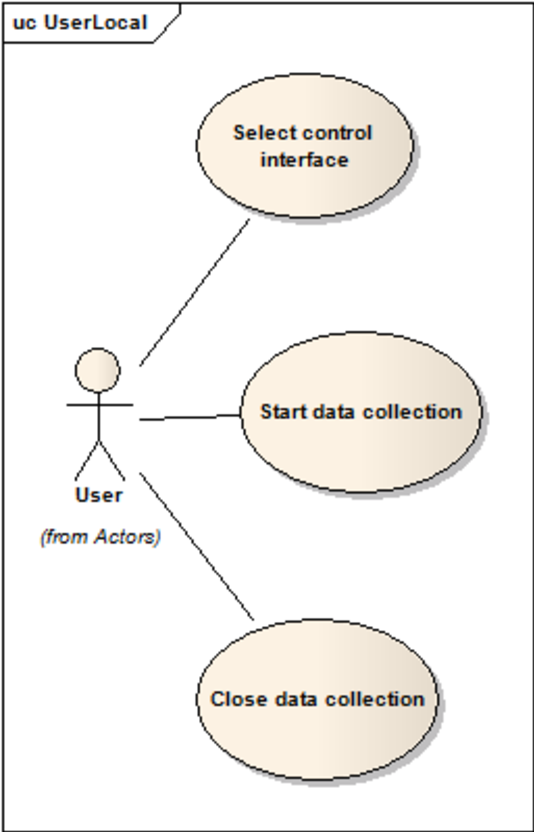
\includegraphics[width=0.75\linewidth]{img/cap4/userCaseLocal}
\caption{User: Local use case} \label{subfig:userCaseLocal}
\end{minipage}
\begin{minipage}{0.45\linewidth}
\center
\captionsetup{justification=centering,margin=0cm,font=small}
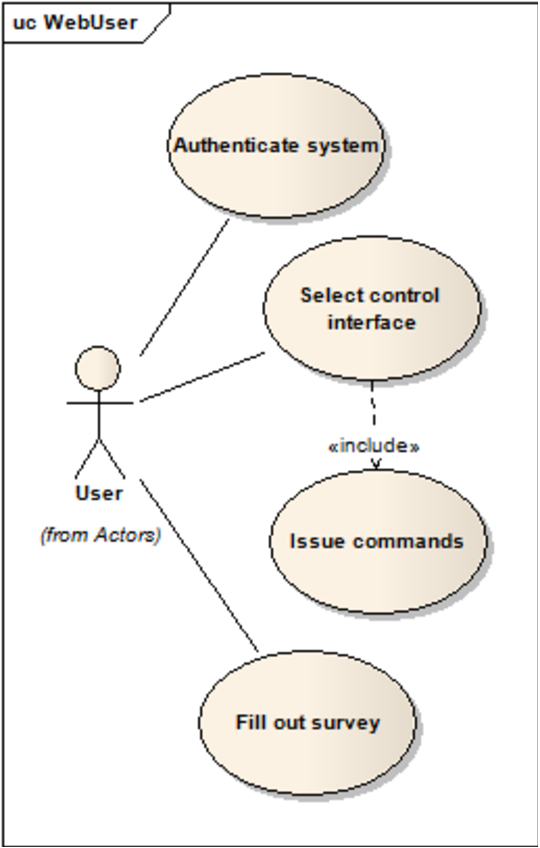
\includegraphics[width=0.75\linewidth]{img/cap4/userCaseWeb}
\caption{User: Web use case} \label{subfig:userCaseWeb}
\end{minipage}
\end{figure}

In order for the therapist to perform his duties through the process of rehabilitation of the PW user, the following actions were established described in Figure \ref{fig:therapistCases}. Thus, the therapist is able to perform the following actions: to record his users' information in the system, create training protocols that meet the needs and capabilities of the individual user, define which protocols will be executed, initiate and monitor the training sessions and, if necessary, intervene in addition to evaluating, taking notes and track the history of training progress for each user. 

In this way, the therapist can perform his activities as if he were inside the rehabilitation center.

\begin{figure}[!hbt]
\begin{center}
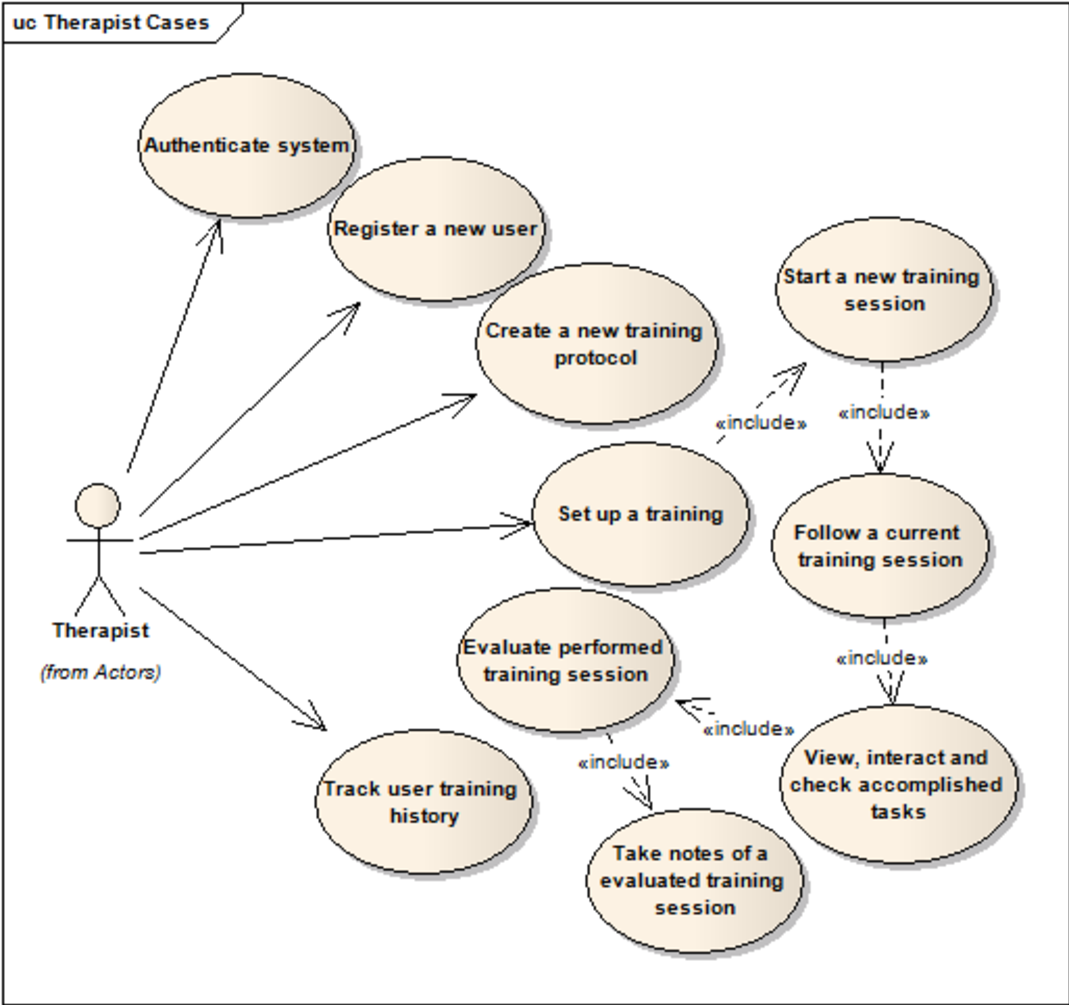
\includegraphics[width=0.55\linewidth]{img/cap4/therapistCases}
\caption{Therapist use case} \label{fig:therapistCases}
\end{center}
\end{figure}

Based on the actions performed by users and therapists, some actions must be made by the system (Figure \ref {fig:systemActionsCase}). These actions ensure that requests are correctly handled, as resources become available. Thus, they can receive the correct feedback of actions remotely performed through remote interactions with PW.

Figure \ref {fig:adminCase} demonstrates some administrative activities, which for the time being, must be defined before using the system, so that the environments are appropriately connected and to have control over the moment of information collection, from the experiences, carried out by users.

\begin{figure}[!htbp]
\center
\begin{minipage}{0.45\linewidth}
\center
\captionsetup{justification=centering,margin=0.5cm,font=small}
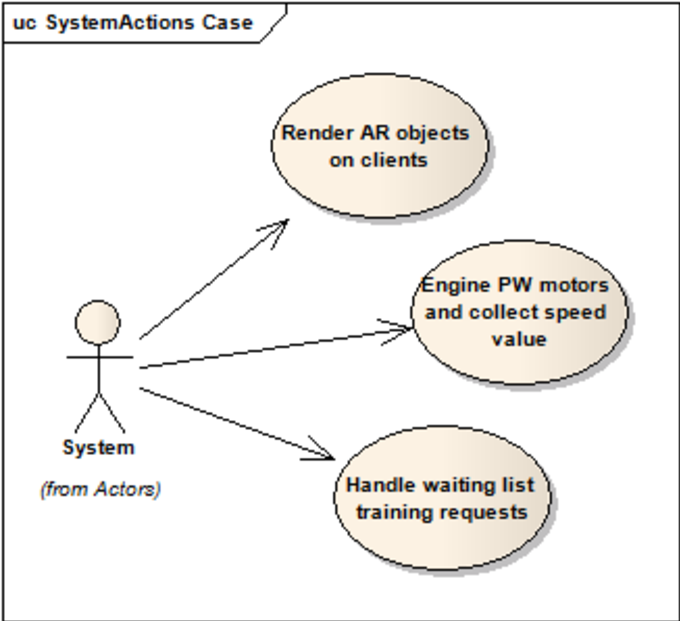
\includegraphics[width=0.93\linewidth]{img/cap4/systemActionsCase}
\caption{System use case} \label{fig:systemActionsCase}
\end{minipage}
\begin{minipage}{0.45\linewidth}
\center
\captionsetup{justification=centering,margin=0cm,font=small}
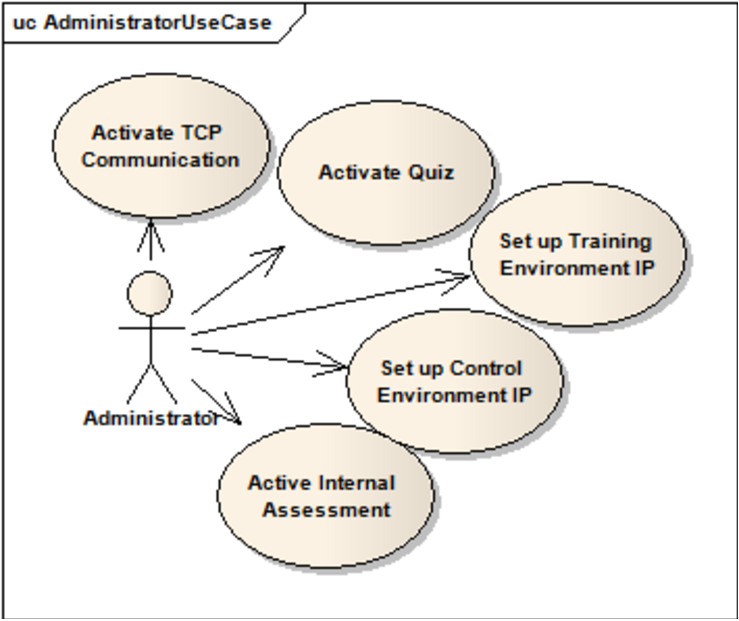
\includegraphics[width=1\linewidth]{img/cap4/adminCase}
\caption{Administrator use case} \label{fig:adminCase}
\end{minipage}
\end{figure}

These requirements are fundamental for the environments in order to provide the user with a more realist environment. Thus, next session presents the proposed system architecture. 

\section{System architecture}

A computational system used to train and evaluate users at a distance is, essentially, composed by three main modules, according to \cite{burdea2004}:

\begin{enumerate}[label=(\alph*)]
\item Exercise software, running on the users station;
\item Remote monitoring software, running on the therapist site; and
\item A database and remote graphics capability, used for user's medical data.
\end{enumerate}

Considering the main needed characteristics, based on previous related work and associating to the description provided by \cite{burdea2004}, the following software system architecture, shown in Figure \ref{fig:architecture} is proposed:

\begin{figure}[!hbt]
\begin{center}
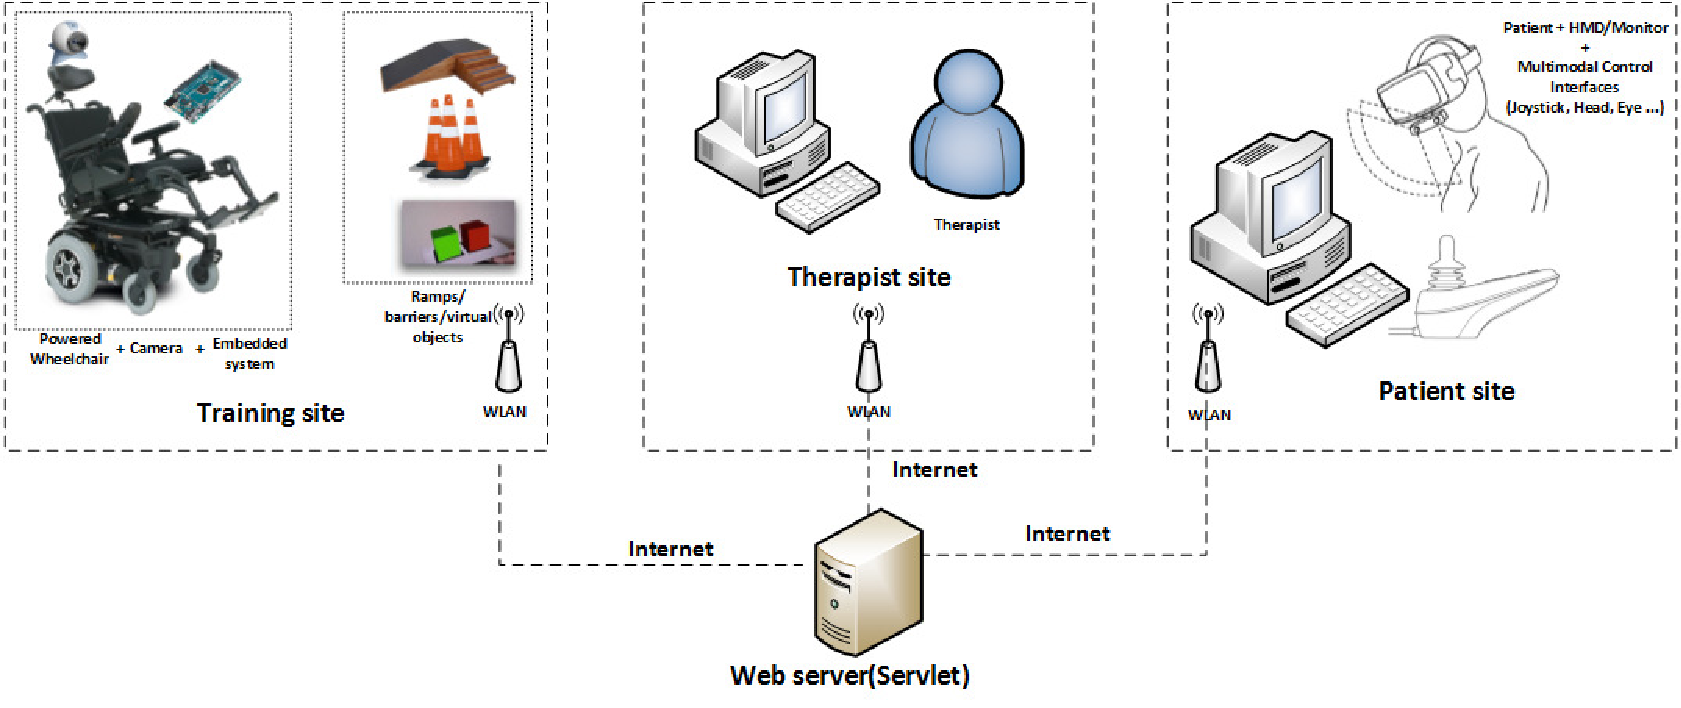
\includegraphics[width=1 \textwidth]{img/cap4/architecture}
\caption{AR Telerehabilitation System Architecture} 
\label{fig:architecture}
\end{center}
\end{figure}


\begin{enumerate}
\item A training site, in which the exercises protocol will be executed, is similar to the one proposed in item (a);
\item A patient site, from which the user remotely controls the PW, is similar to the one proposed in item (a); and
\item A therapist site is similar to those proposed in itens (b) and (c), in which a health professional can follow the exercises executed by the user and access performance data.
\end{enumerate}

The following sections, explain the main details about each site.

\section{System sites}

\subsection{Training site}

This site is a controlled environment where each structural part was built based on 60 surveys form (Appendix I) filled out by PW users with different disabilities. The area presented in Figure \ref{fig:roomView} is 14.76x7.16m$^{2}$ and is located in a classroom (-18.944766, -48.213257) at the Federal University of Uberlândia. 


\begin{figure}[!hbt]
\begin{center}
\includegraphics[width=1 \textwidth]{img/cap4/roomView}
\caption{Remote training site} 
\label{fig:roomView} 
\end{center}
\vspace{-20pt}
\end{figure}


The room is composed by an unmanned PW (Figure \ref{fig:wheel-smbsm2}) without diagonal movements, physical objects such as curb and a high access ramp, uneven surface area, spine, portal and a set of AR markers,  equally spaced a meter apart from each other. 

\begin{figure}[!hbt]
\begin{center}
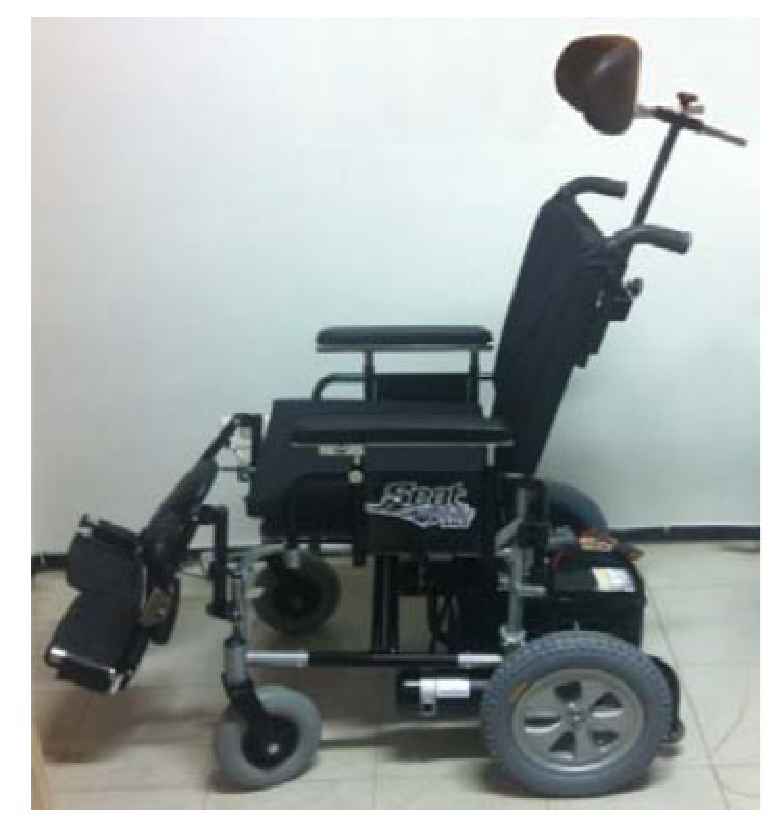
\includegraphics[width=0.4\textwidth]{img/cap4/wheel-smbsm2}
\caption{PW vehicle}
\label{fig:wheel-smbsm2}
\end{center}
\vspace{-20pt}
\end{figure}

The AR markers matrix has 14x7 positions. Additionally, virtual objects will be positioned over the AR markers, according to the configuration proposed by the therapist. From a Dlink DWR-922B 4G router modem (Figures \ref{fig:routerDWR922b4g-front} and \ref{fig:routerDWR922b4g-back}), controlled through a connect to the Internet.

\begin{figure}[!htbp]
\center
\begin{minipage}{0.45\linewidth}
\center
\captionsetup{justification=centering,margin=0cm,font=small}
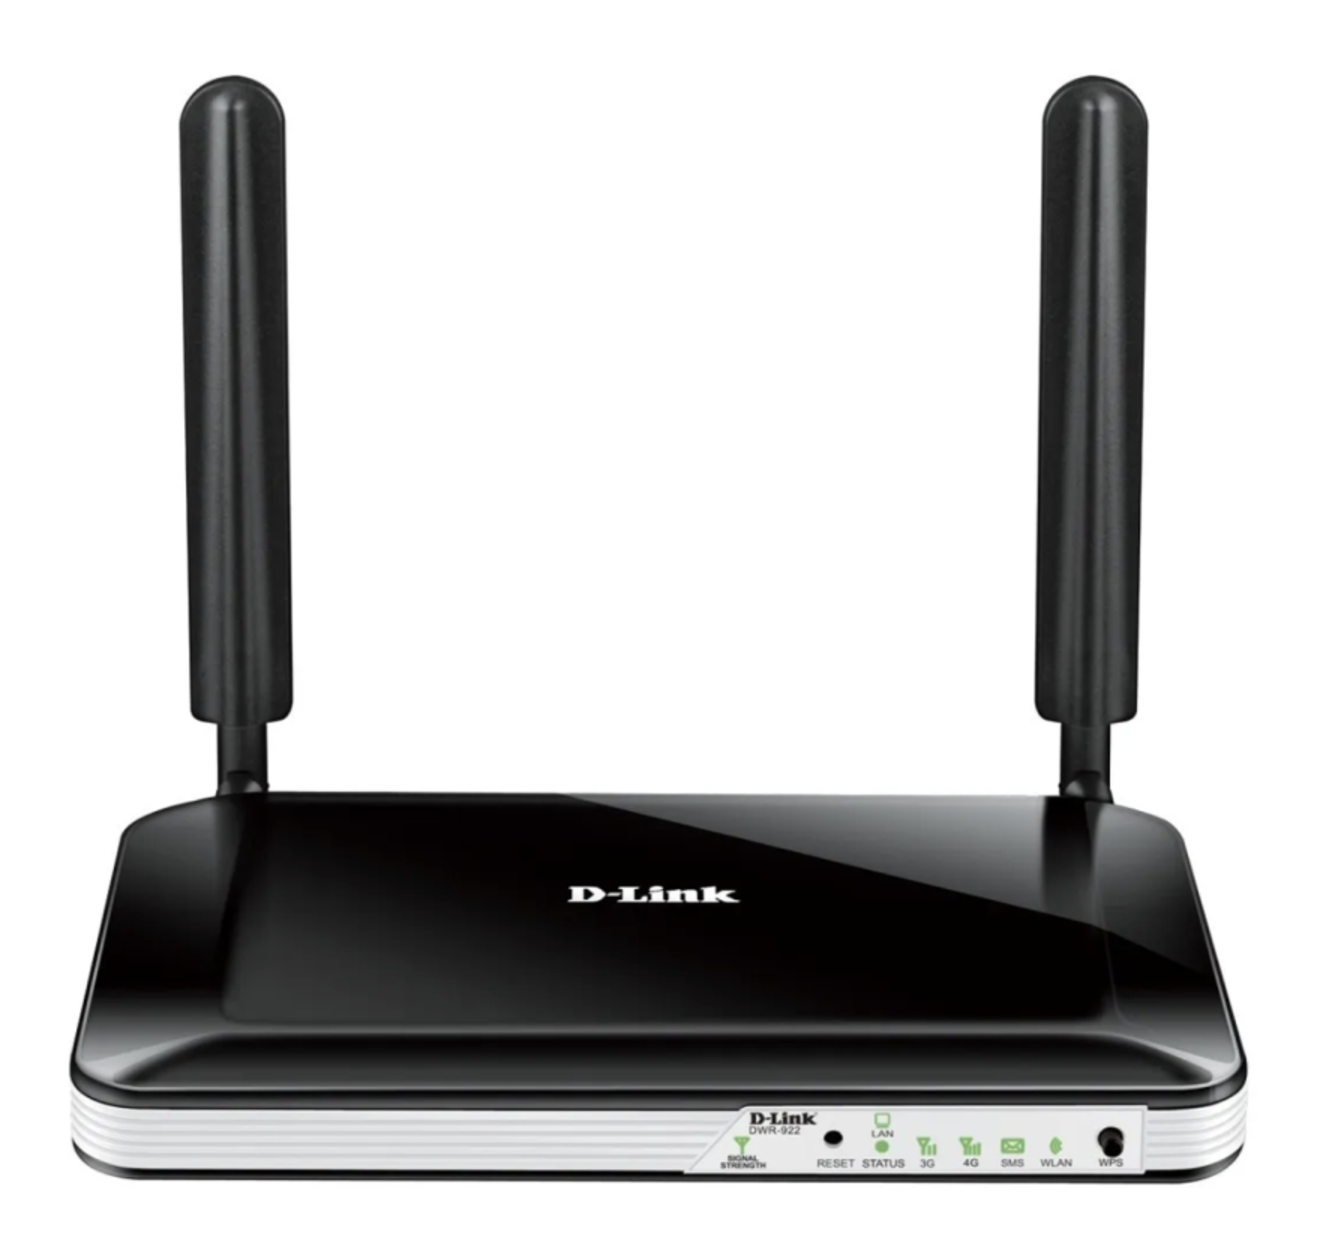
\includegraphics[width=0.8\linewidth]{img/cap4/routerDWR922b4g-front}
\caption{Dlink DWR-922B - Front} \label{fig:routerDWR922b4g-front}
\end{minipage}
\begin{minipage}{0.45\linewidth}
\center
\captionsetup{justification=centering,margin=0cm,font=small}
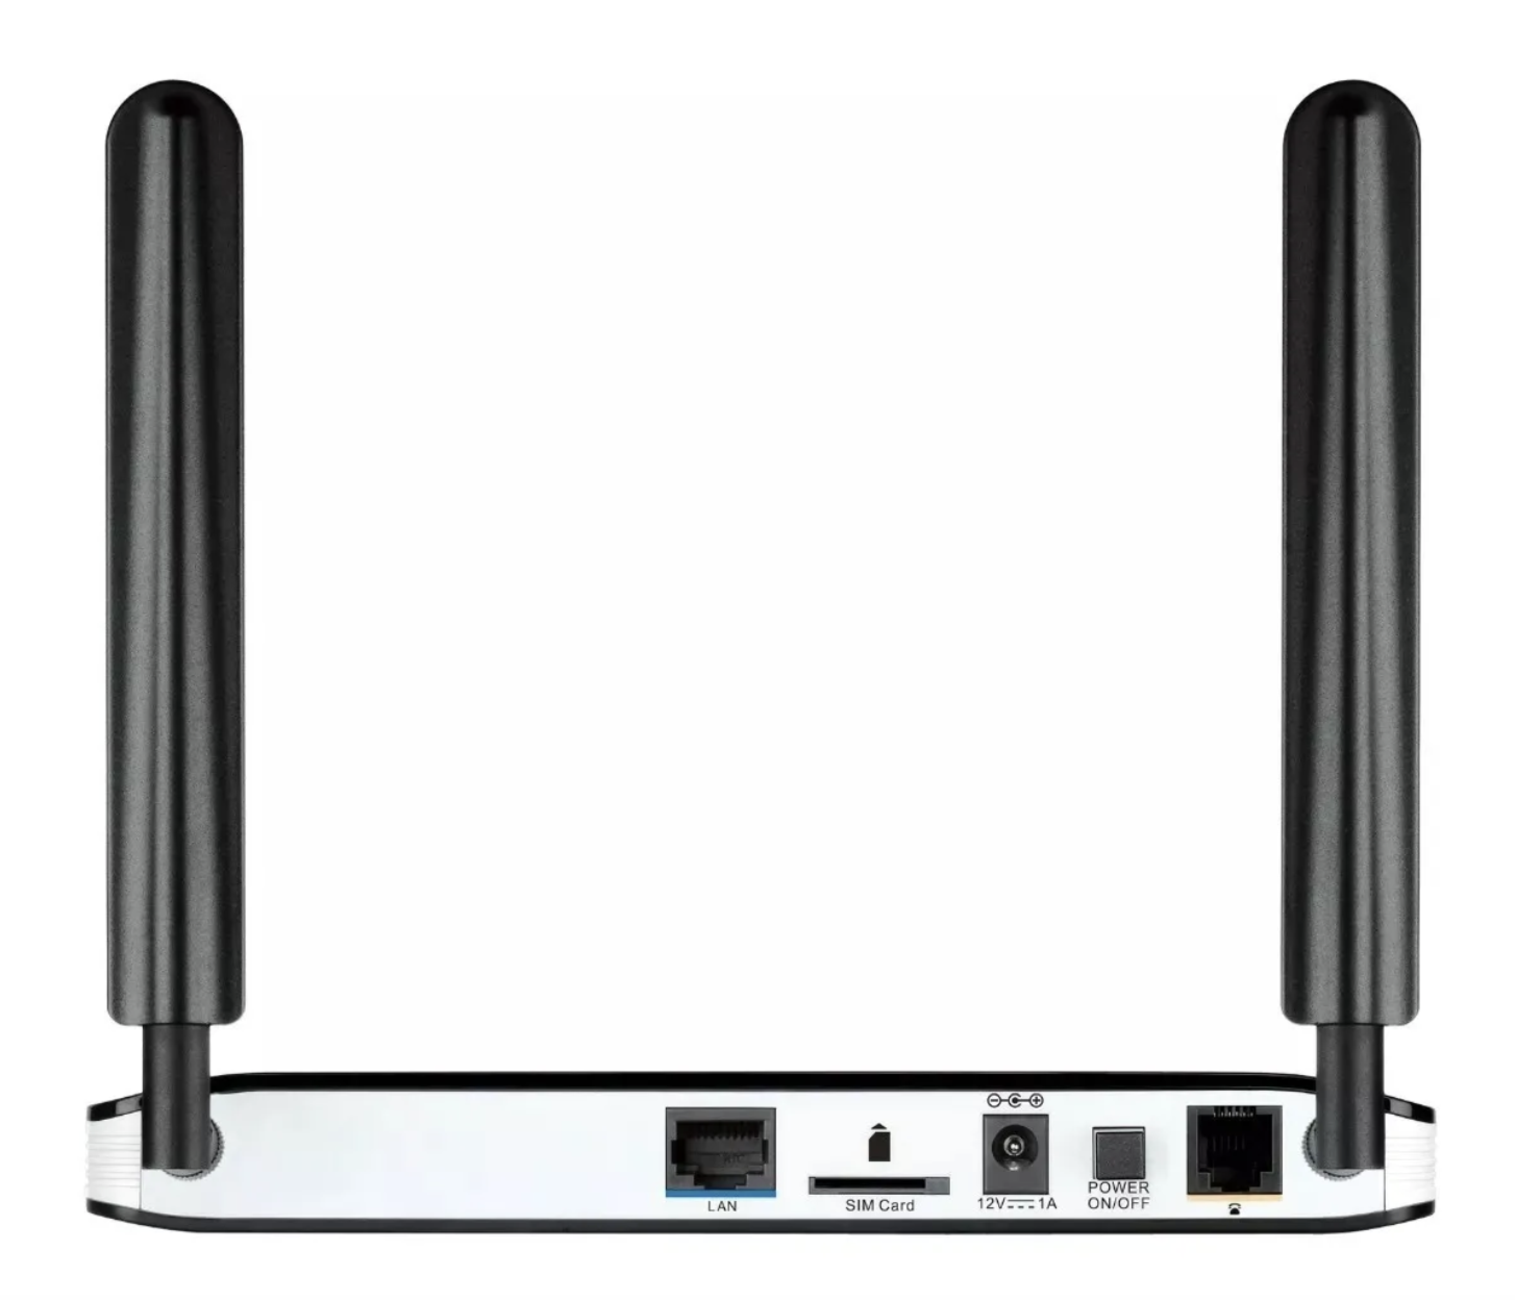
\includegraphics[width=0.88\linewidth]{img/cap4/routerDWR922b4g-back}
\caption{Dlink DWR-922B - Back} \label{fig:routerDWR922b4g-back}
\end{minipage}
\end{figure}

An interface controller box (Figure \ref{fig:controllerInterfaceBox-front} and \ref{fig:controllerInterfaceBox-back}) are coupled to the PW (Figure \ref{fig:controllerBox-external} and \ref{fig:controllerBox-internal}) to trigger motor and collect the PW speed. The  internal components of Figure \ref{fig:controllerBox-internal} are: 1) Proprietary board under interface panel, 2) Input signals (Arduino) plug, 3) Processed control signals, 4) Internal power supply cables and 5) PW driver plug.


\begin{figure}[!htbp]
\center
\begin{minipage}{0.495\linewidth}
\center
\captionsetup{justification=centering,margin=0cm,font=small}
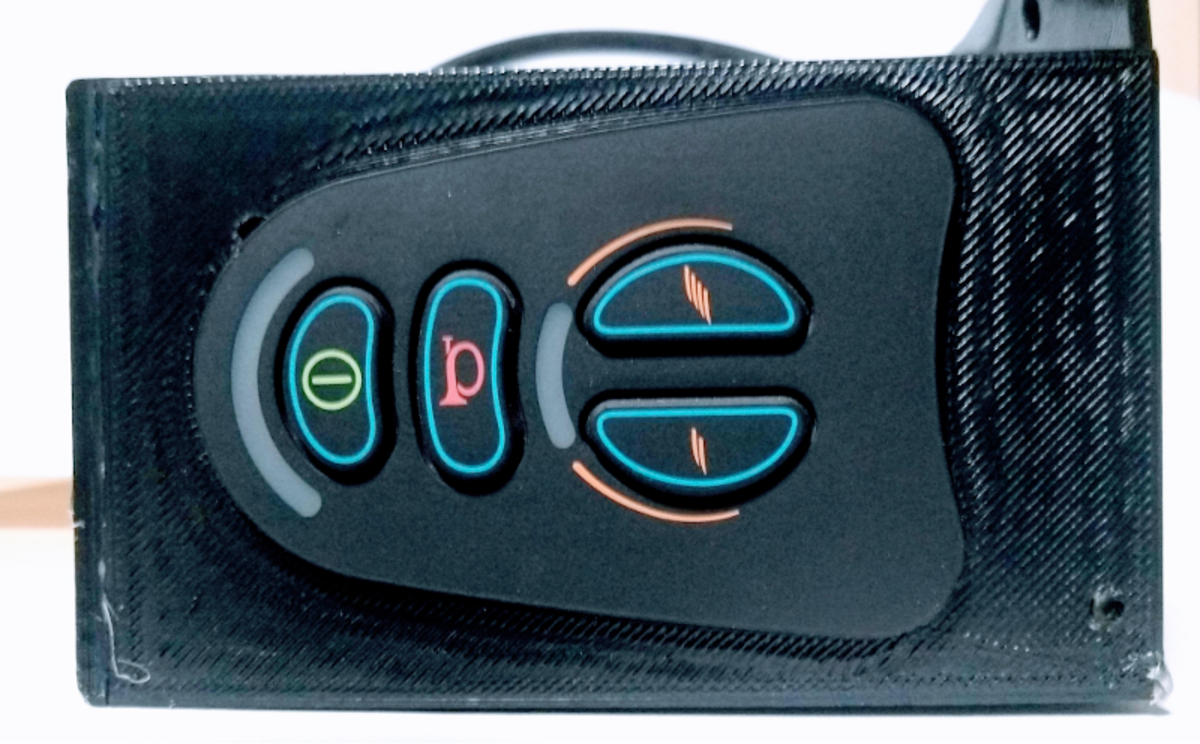
\includegraphics[width=0.85\linewidth]{img/cap4/controllerInterfaceBox-front}
\caption{HMI PW (Front): only Power On/Off interface panel option} \label{fig:controllerInterfaceBox-front}
\end{minipage}
\begin{minipage}{0.495\linewidth}
\center
\captionsetup{justification=centering,margin=0cm,font=small}
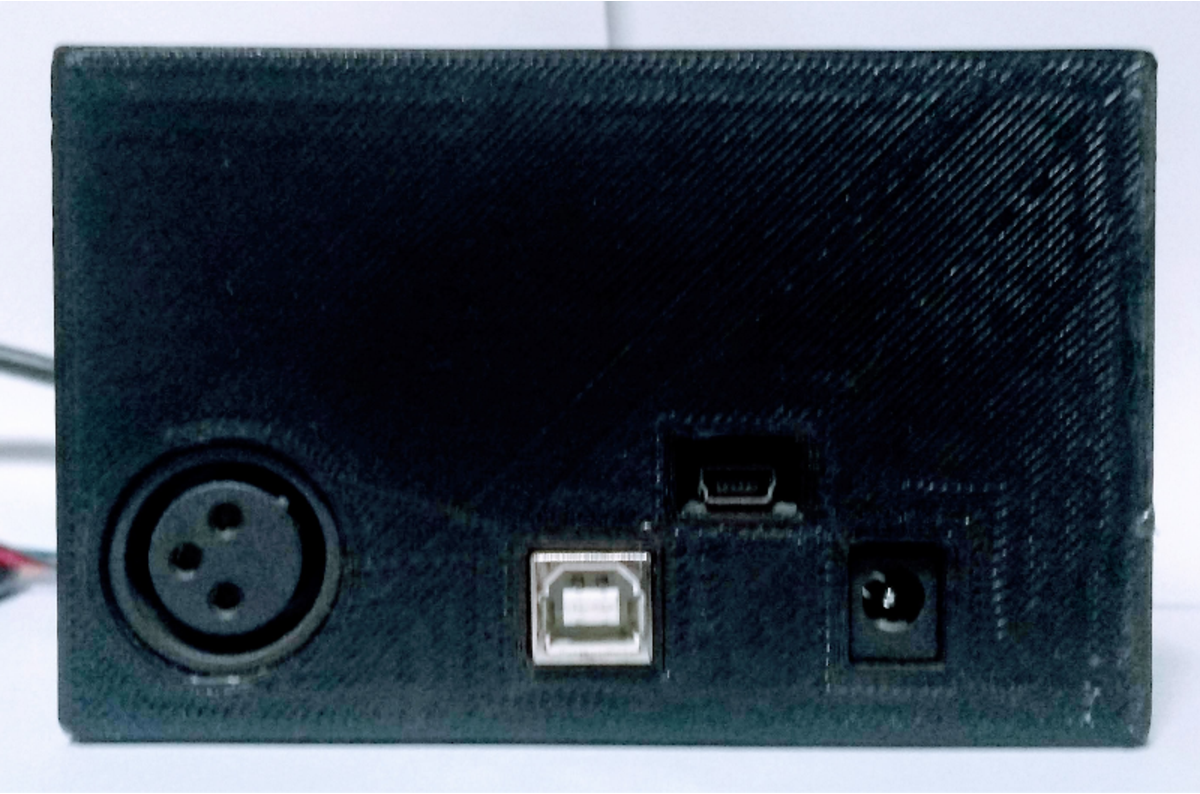
\includegraphics[width=0.8\linewidth]{img/cap4/controllerInterfaceBox-back}
\caption{HMI PW (Back): PW and Arduino power supply plugs} \label{fig:controllerInterfaceBox-back}
\end{minipage}
\end{figure}


\begin{figure}[!htbp]
\center
\begin{minipage}{0.495\linewidth}
\center
\captionsetup{justification=centering,margin=0cm,font=small}
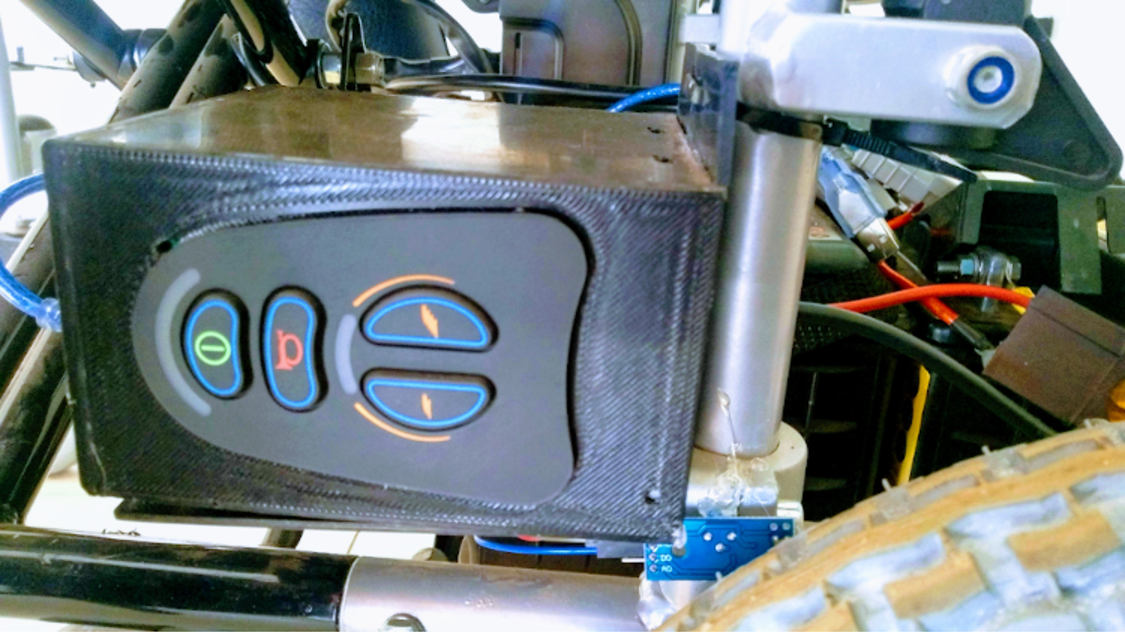
\includegraphics[width=0.9\linewidth]{img/cap4/controllerBox-external}
\caption{Control box position at PW} \label{fig:controllerBox-external}
\end{minipage}
\begin{minipage}{0.495\linewidth}
\center
\captionsetup{justification=centering,margin=0cm,font=small}
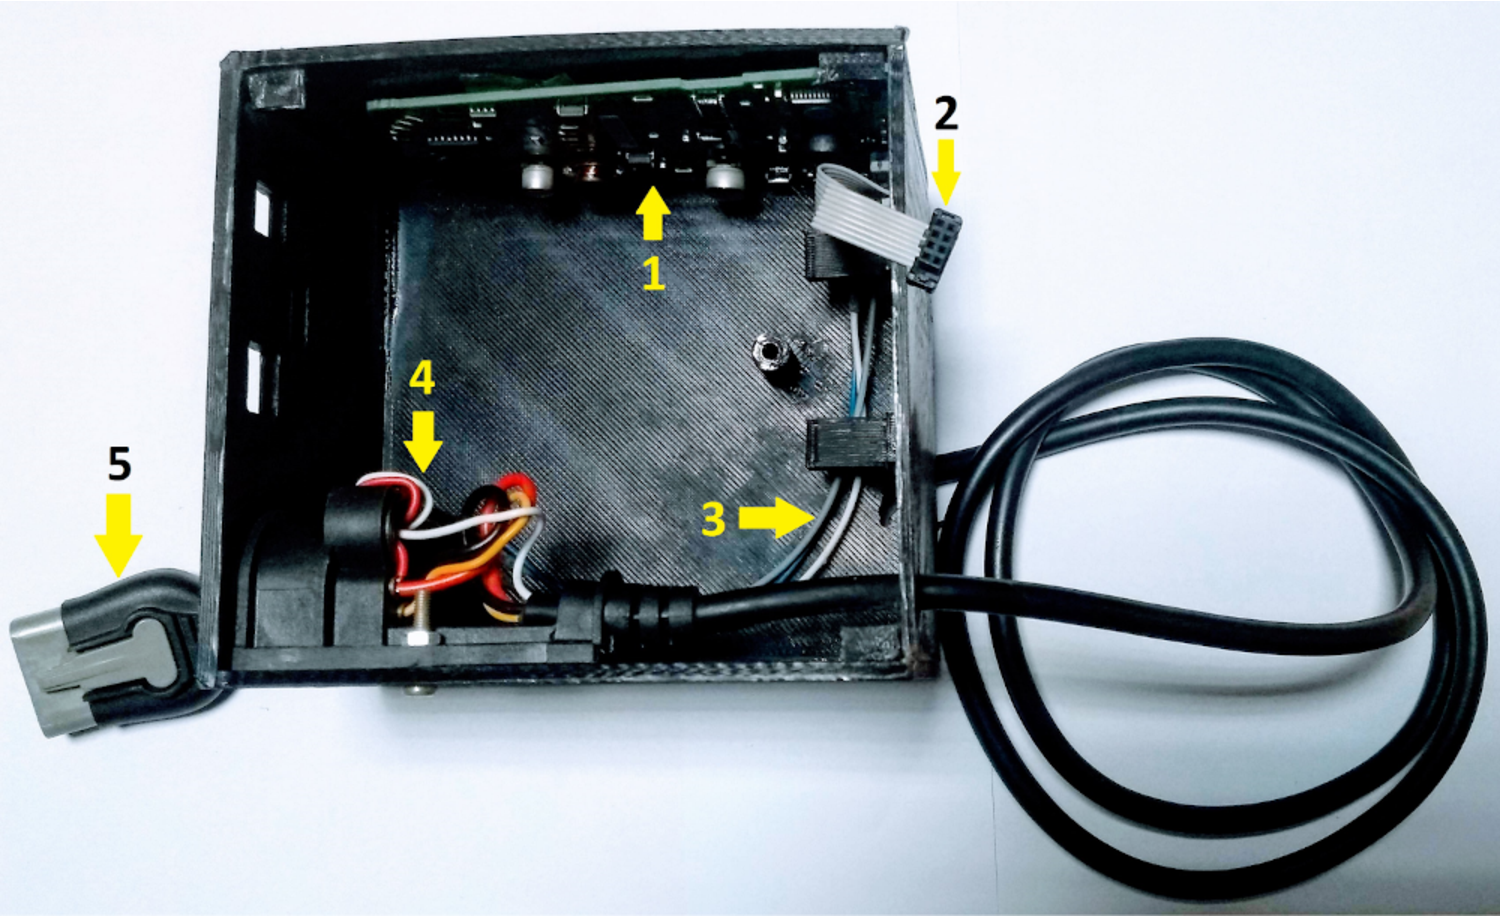
\includegraphics[width=0.85\linewidth]{img/cap4/controllerBox-internal}
\caption{ Internal control box components*} \label{fig:controllerBox-internal}
\end{minipage}
\end{figure}

A smartphone is integrated into the PW to provide remote clients (users and therapists) with visual feedback. These clients have, in their respective sites, a vision in the first-person of the augmented training session, which is more natural and realistic against the god view mode, which gives the user a top view of the whole environment. Also, the smartphone running the  Android operating system, has a Team Viewer QuickSupport app installed to afford a remote connection.

\subsubsection{PW control and Speed signal collection }

A microcontroller board Arduino Mega 2560\footnote{https://www.arduino.cc/en/Main/arduinoBoardMega} (Figure \ref{subfig:arduino-mega2560})  within a wifiShield\footnote{https://www.arduino.cc/en/Main/ArduinoWiFiShield} (Figure \ref{subfig:arduino-wifishield}) is used to load the embedded system which receives all commands through the Wireless Local Area Network  (WLAN) network. 

\begin{figure}[!htbp]
\center
\begin{minipage}{0.4\linewidth}
\center
\captionsetup{justification=centering,margin=0.5cm,font=small}
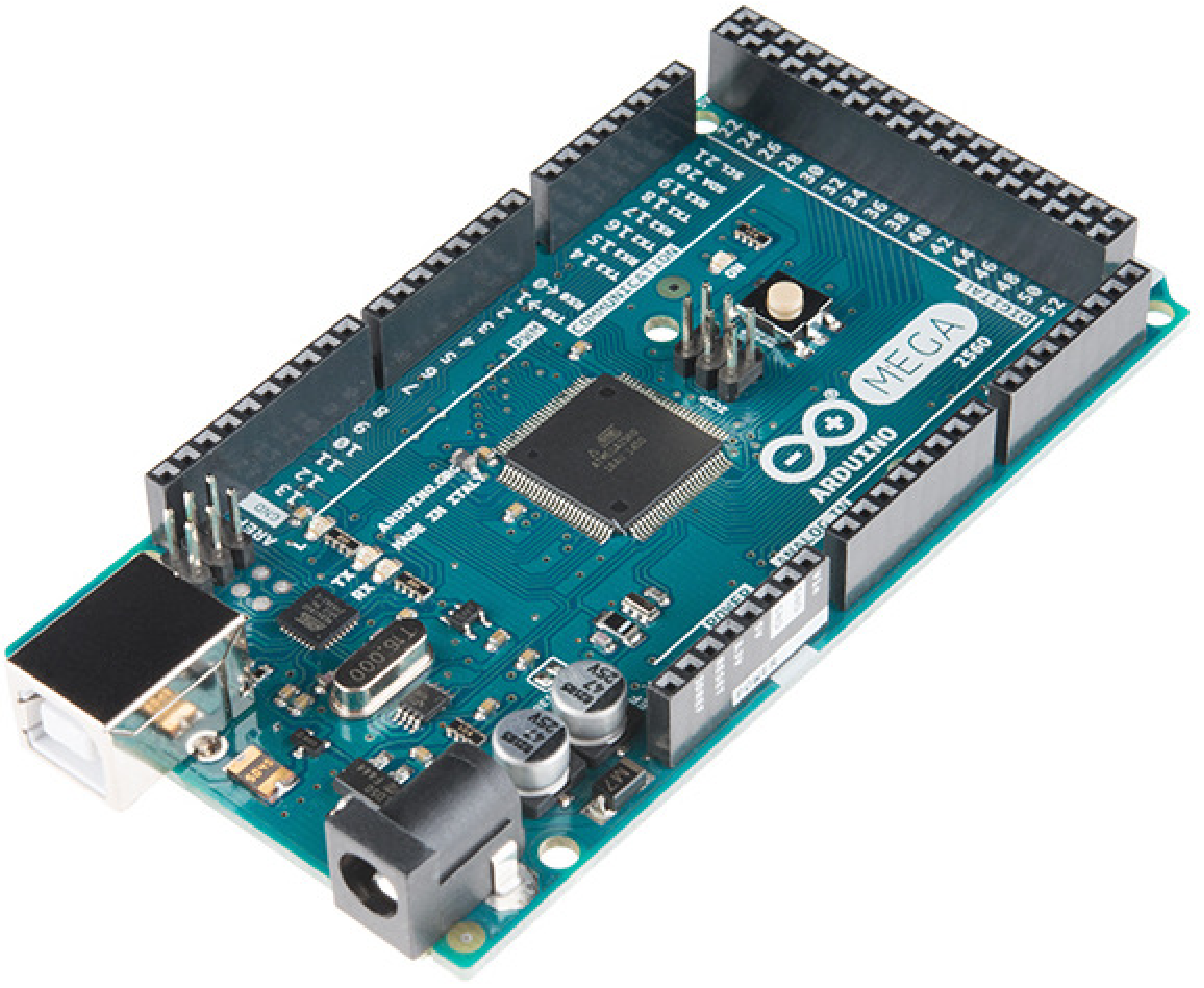
\includegraphics[width=0.87 \linewidth]{img/cap4/arduino-mega2560}
\caption{Arduino Mega 2560} \label{subfig:arduino-mega2560}
\end{minipage}
\begin{minipage}{0.4\linewidth}
\center
\captionsetup{justification=centering,margin=0cm,font=small}
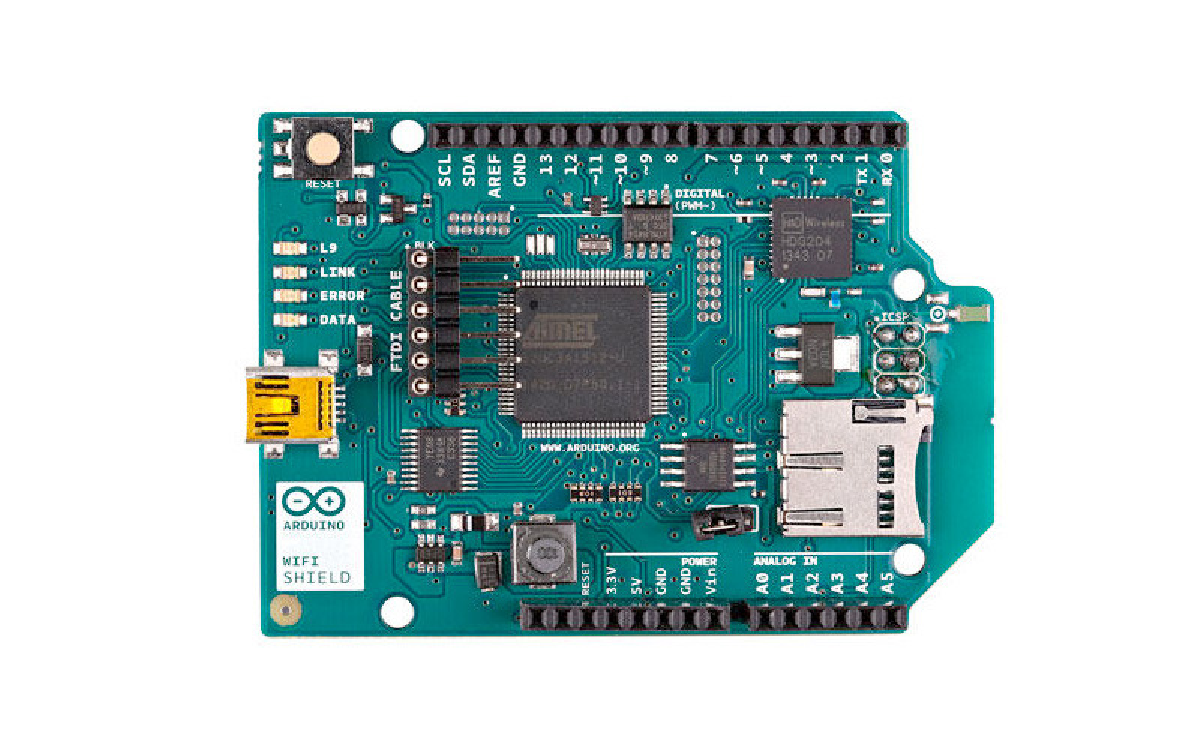
\includegraphics[width=1.15\linewidth]{img/cap4/arduino-wifishield}
\caption{WifiShield Arduino} \label{subfig:arduino-wifishield}
\end{minipage}
\end{figure}

A  PWM shield  (Figure \ref{fig:pwcontrollershield}) is used to transcript control signals, remotely received in different PWM pulses, which are recognised by proprietary board in Figure \ref{fig:controllerBox-internal}, responsible, in turn, to engine PW. The sensor (Figure \ref{fig:speedsensor}) responsible for collecting the PW speed are coupled to it. The PW is controlled by an embedded system, which receives control signals from the remote server that is responsible for forwarding each signal received from the user. Control signals are received from the Internet and sent through a WLAN that returns the PW speed values to the remote server.


\begin{figure}[!htbp]
\center
\begin{minipage}{0.495\linewidth}
\center
\captionsetup{justification=centering,margin=0.5cm,font=small}
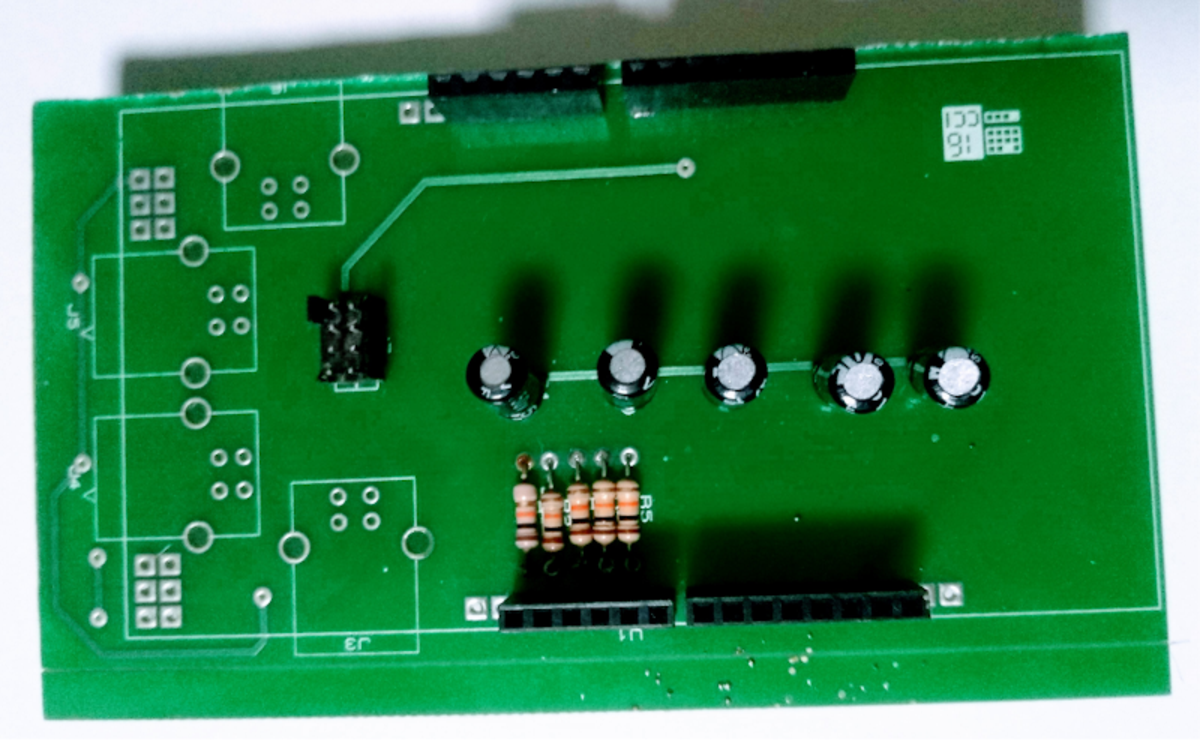
\includegraphics[width=0.95\linewidth]{img/cap4/pwcontrollershield}
\caption{PWM Shield converter} \label{fig:pwcontrollershield}
\end{minipage}
\begin{minipage}{0.495\linewidth}
\center
\captionsetup{justification=centering,margin=0cm,font=small}
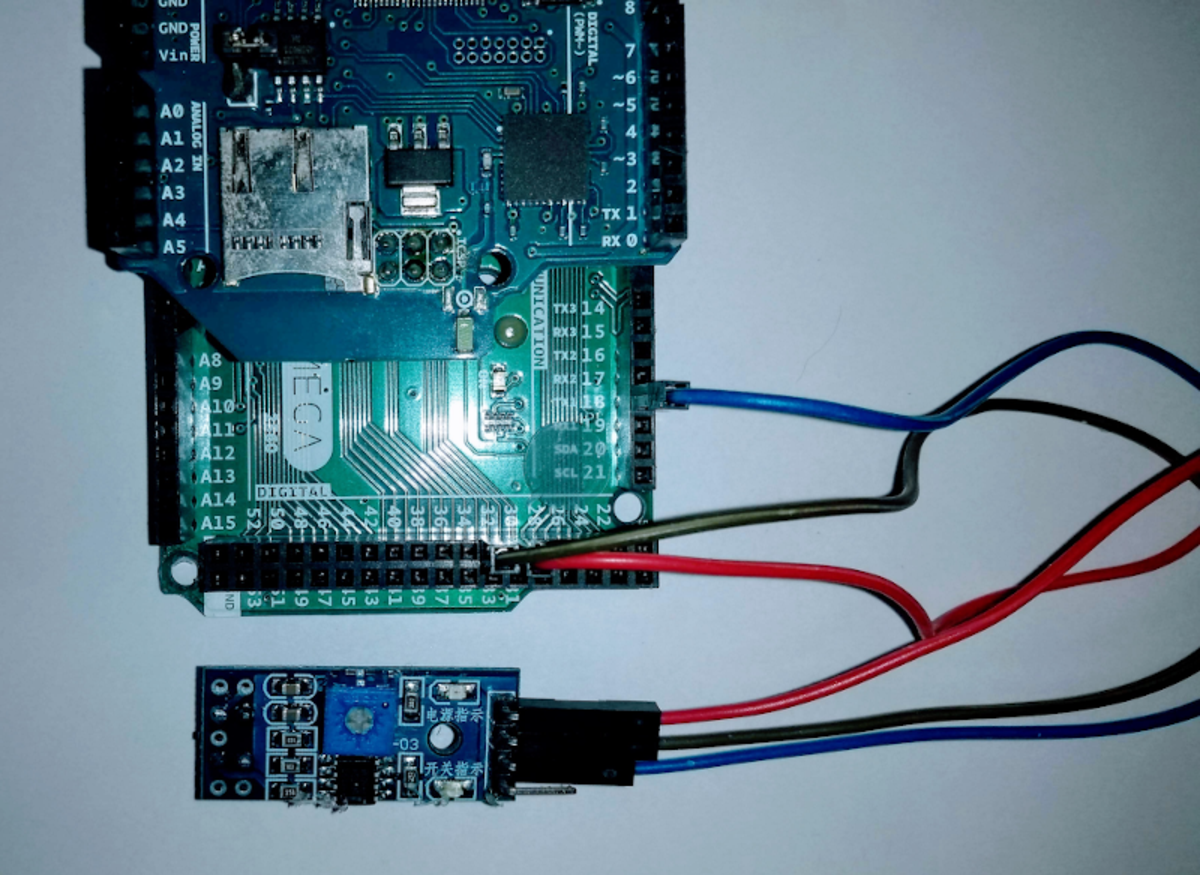
\includegraphics[width=0.8\linewidth]{img/cap4/speedsensor}
\caption{Sensor follow infrared range IR Tcrt5000 Lm393} \label{fig:speedsensor}
\end{minipage}
\end{figure}

Through the WLAN, a data channel is established between patients and the training site. The command data streaming is released only after the user training request be authorized by the therapist. After that, an algorithm capable of recognizing each command and performing the respective PW movement is uploaded into the microcontroller. Nevertheless, for many reasons, sometimes, the control inputs can not be received because the data channel connection may fall or some package may be lost. For this reason, an emergency stop must be defined to avoid some possible PW crash \cite{mitsumura2014}. Figure \ref{fig:wheelChairActivity} presents a Unified Modeling Language (UML) Activity Diagram of this process workflow.

\begin{figure}[!hbt]
\begin{center}
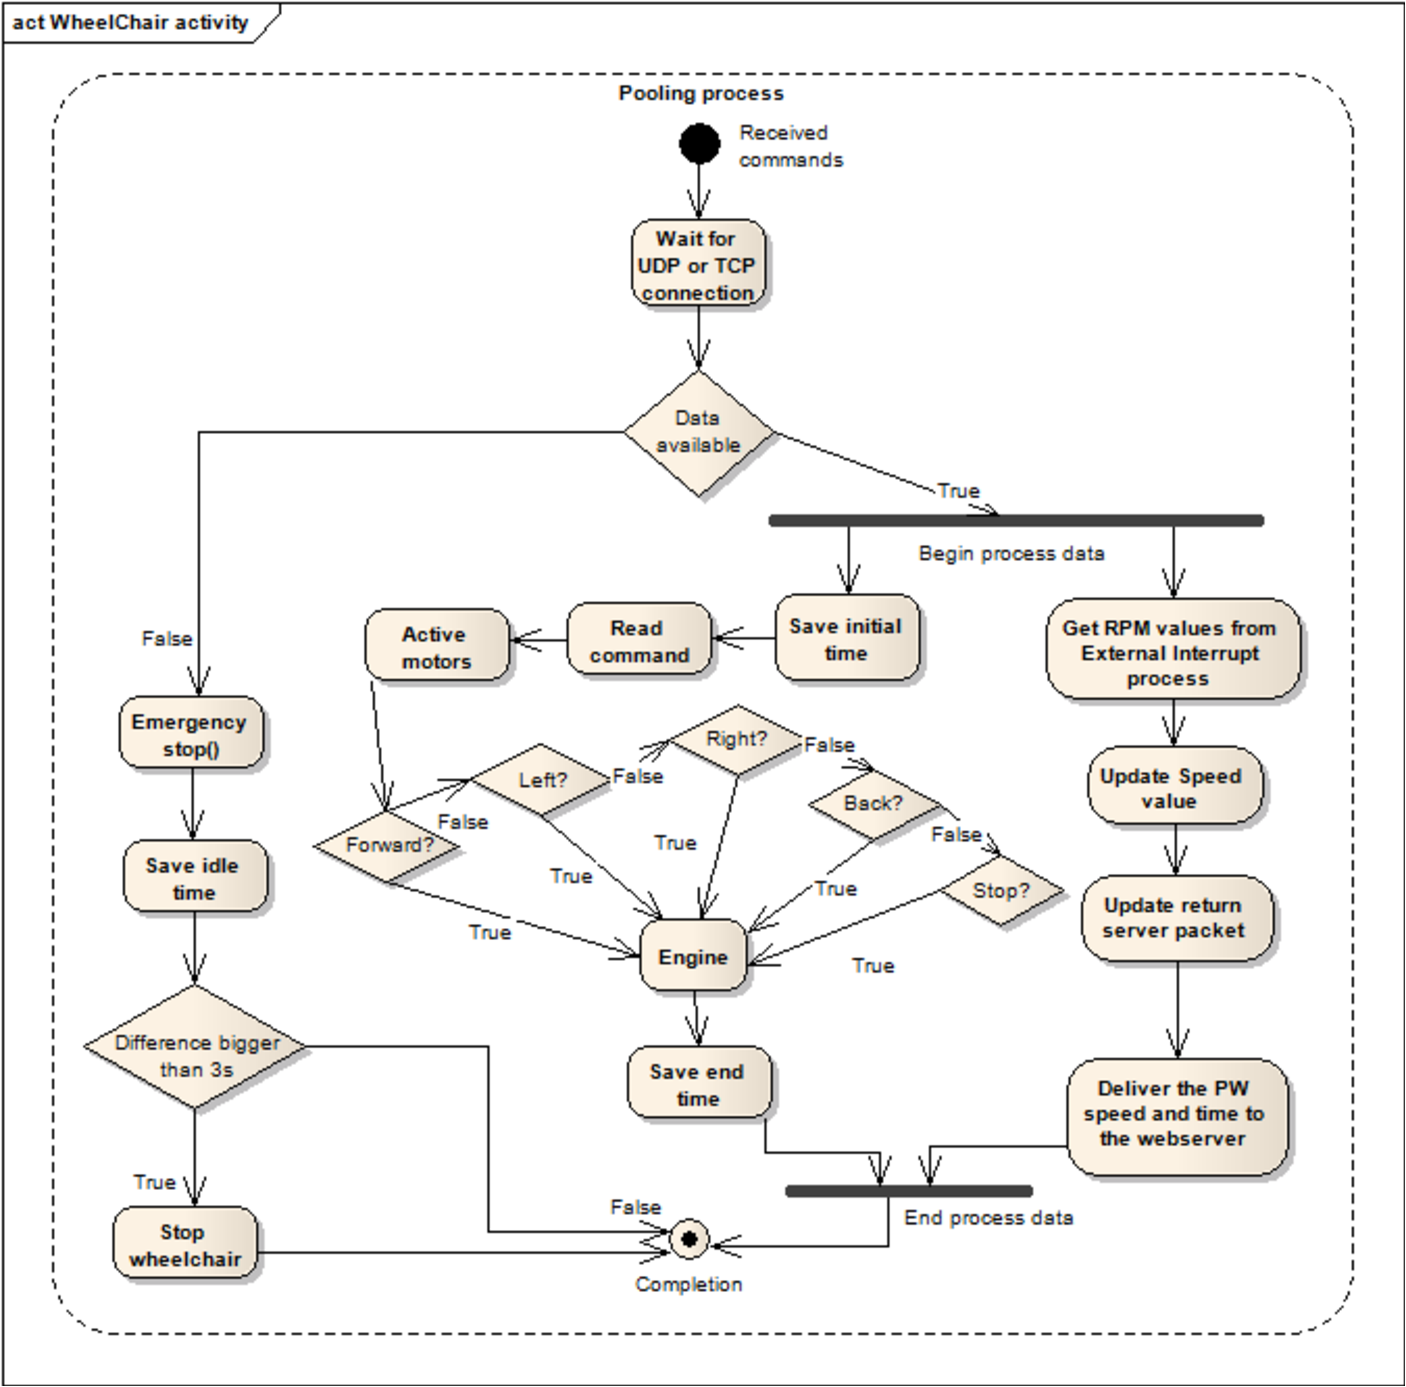
\includegraphics[width=0.9 \textwidth]{img/cap4/wheelChairActivity}
\caption{Activity Diagram to PW data workflow} 
\label{fig:wheelChairActivity}
\end{center}
\end{figure}

This Activity Diagram describes all actions related to data workflow into the embedded software. The microcontroller has the primary function of running all the time (pooling process) and also an interrupt process attached at the speed sensor, responsible for updating the PW Revolutions Per Minute (RPM). The first step is to recognize the client connection and if it has some data to be processed. Currently, this data is represented by a string value like (1, 2, 3, 4, or 5)\cite{caetano2018}.  The PW, at this point, is only working with continuous speed. Further, the speed value can be changed in the agreement with PW user needs.  The second step is, if it has data available, the initial time is updated and a general method accountable for activating the PW motors is triggered by performing the respective movement. Also, the RPM speed values are converted by Km/h values and buffered in a data packet. Otherwise, if it has no data available, the security function is called. Thus, the idle time is updated. After, the time difference between idle and initial is checked, and if it's bigger than 3 seconds, the general wheelchair method is called to stop the PW. In the end, a data packet containing microcontroller internal processing time information and the speed of the PW is returned to the server.

\subsection{Patient  site}
\label{sec:controlenv}

In this  site, the user is able to issue control commands to the remote PW, using the adapted joystick, as shown in Figure \ref{fig:USBjoystickvr2}. Visual feedback is provided to the user.

\begin{figure}[!hbt]
\begin{center}
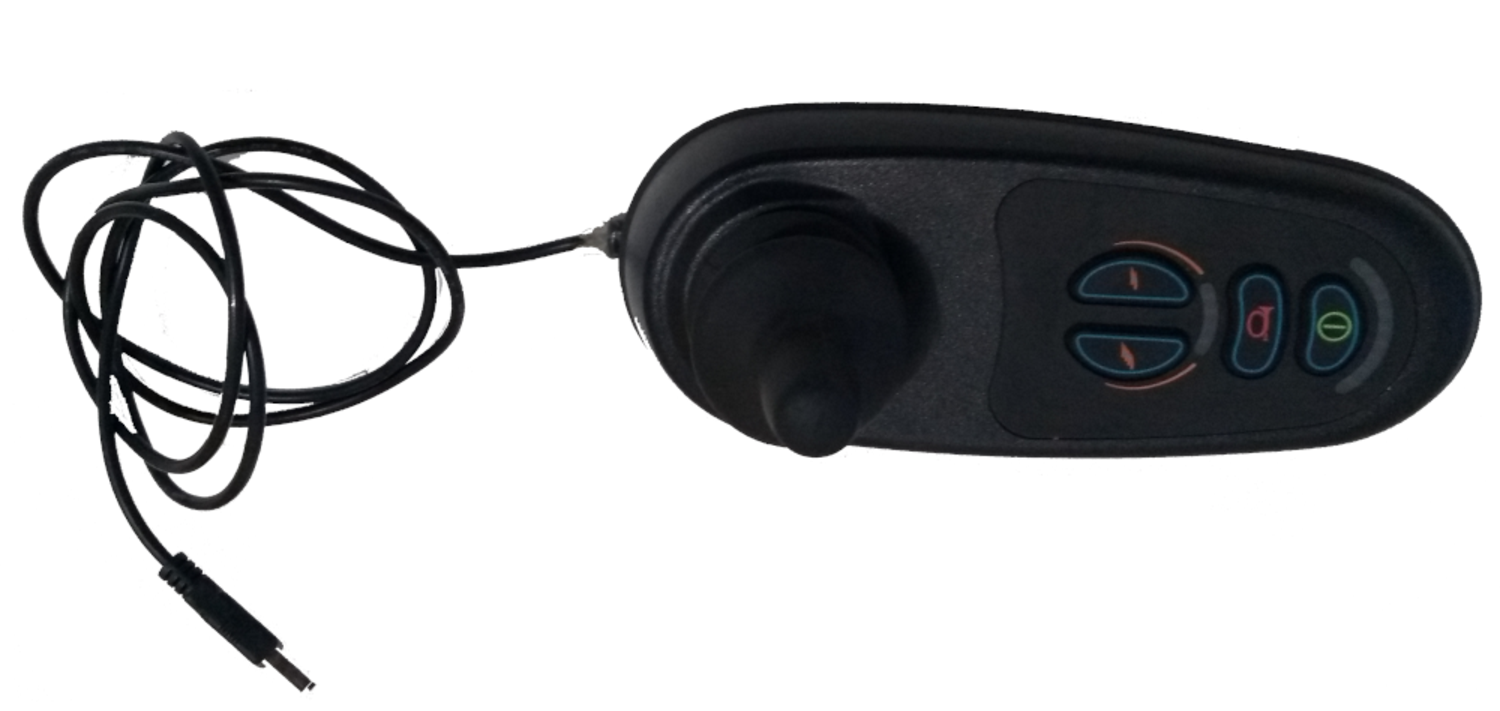
\includegraphics[width=1 \textwidth]{img/cap4/USBjoystickvr2}
\caption{Adapted USB Joystick VR2 \cite{caetano2018}} 
\label{fig:USBjoystickvr2}
\end{center}
\end{figure}

A  desktop computer is used to provide communication with the user. Control commands are collected and further sent to the remote server, which is responsible to forward each command to the training site. Images from the training site are received through the Internet is augmented (AR techniques) and projected on the visual feedback device like a traditional monitor.


\subsection{Therapist site}
\label{sec:supersionenv}

When dealing with telerehabilitation applications, it is desirable that therapists can follow the execution of the exercises \cite{burdea2004}. In the presented architecture, this requirement can be achieved in the therapist site. In this site, the therapist uses a  desktop computer to follow the execution of the exercises by the user from an augmented (AR techniques) visual feedback rendered in his monitor. Also, the therapist would be able to configure the virtual objects to be rendered over the AR markers to customize the set of activities according to users' development in the training process. The therapist has to mark the tasks accomplished by the user during the trial. In the end, the therapist is redirected to an evaluation form to assess the training performed by the user. After the evaluation, the therapist is invited to take clinical notes about the user's experiment and then the evaluation process is finished. At any time, the therapist can access the graphical summary related to the protocols metrics, previously performed by the user.


\section{PMRT methodology}
\label{sec:pmrtmethods}

\subsection{Protocol tasks adaptation}
\label{sec:protocoTadaptation}

The PMRT model, defined  Section in Section \ref{sec:pwTraining}, has being adopted as the standard protocol methodology in this research, due to its reliability. However, the PMRT has 16 tasks structured (predictable) and unstructured (unpredictable). As highlighted by Valentini et al. \cite{valentini2019} the users present themselves tired after accomplishing 12 tasks. Thus, an adaptation on PMRT is required to reduce user mental struggle and achieve his/her goal individually, ensuring his/her well being after the trials.

Data information collected during the trials is shown in Table \ref{table:tbDataCollec}. 


\begin{table}[!hbt]
\caption{Data collection information}\label{table:tbDataCollec}
\centering
\begin{tabular}{ >{\centering}m{0.5cm}  >{}m{14.5cm} }
\toprule
N$^{o}$. &  Description \\
\midrule
1  	& Parameters like the number of input controls, elapsed time, collisions number are used to evaluate the users' trials performance;  \\ \hline
2 	& A survey questionnaire is also used to provide qualitative information about the system from the users point of view as well as the therapist's comments about each activity performed and; \\ \hline
3 	& User biosignals are used to analyze protocols impacts during the trials.\\
\bottomrule
\end{tabular}
\end{table}

\subsection{Biosignal data acquisition and processing}
\label{sec:biosig}
Biosignal data acquisition is performed using the E4 wristband (Figure \ref{fig:e4wristband}), manufactured by Empatica\textregistered. This instrument is an easy to wear wristband that can measure various biosignals, among them Electrodermal Activity (EDA) and Blood Volume Pulse (BVP).

\begin{figure}[!hbt]
\begin{center}
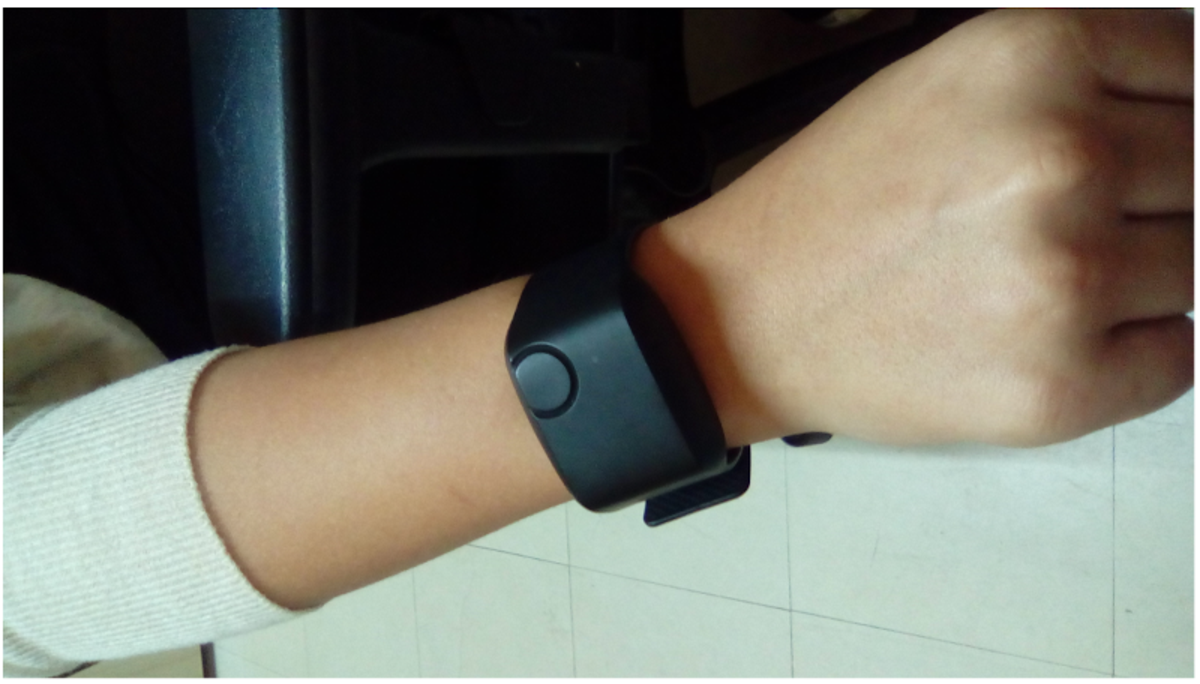
\includegraphics[width=0.8 \textwidth]{img/cap4/e4wristband}
\caption{The E4 wristband for biosignal data acquisition} \label{fig:e4wristband}
\end{center}
\end{figure}


EDA data processing is conducted using Ledalab software \cite{ledalab2020,e4recom2020} to decompose the signal in two components: phasic and tonic (as shown in Figure \ref{fig:ledalab}). 


\begin{figure}[!hbt]
\begin{center}
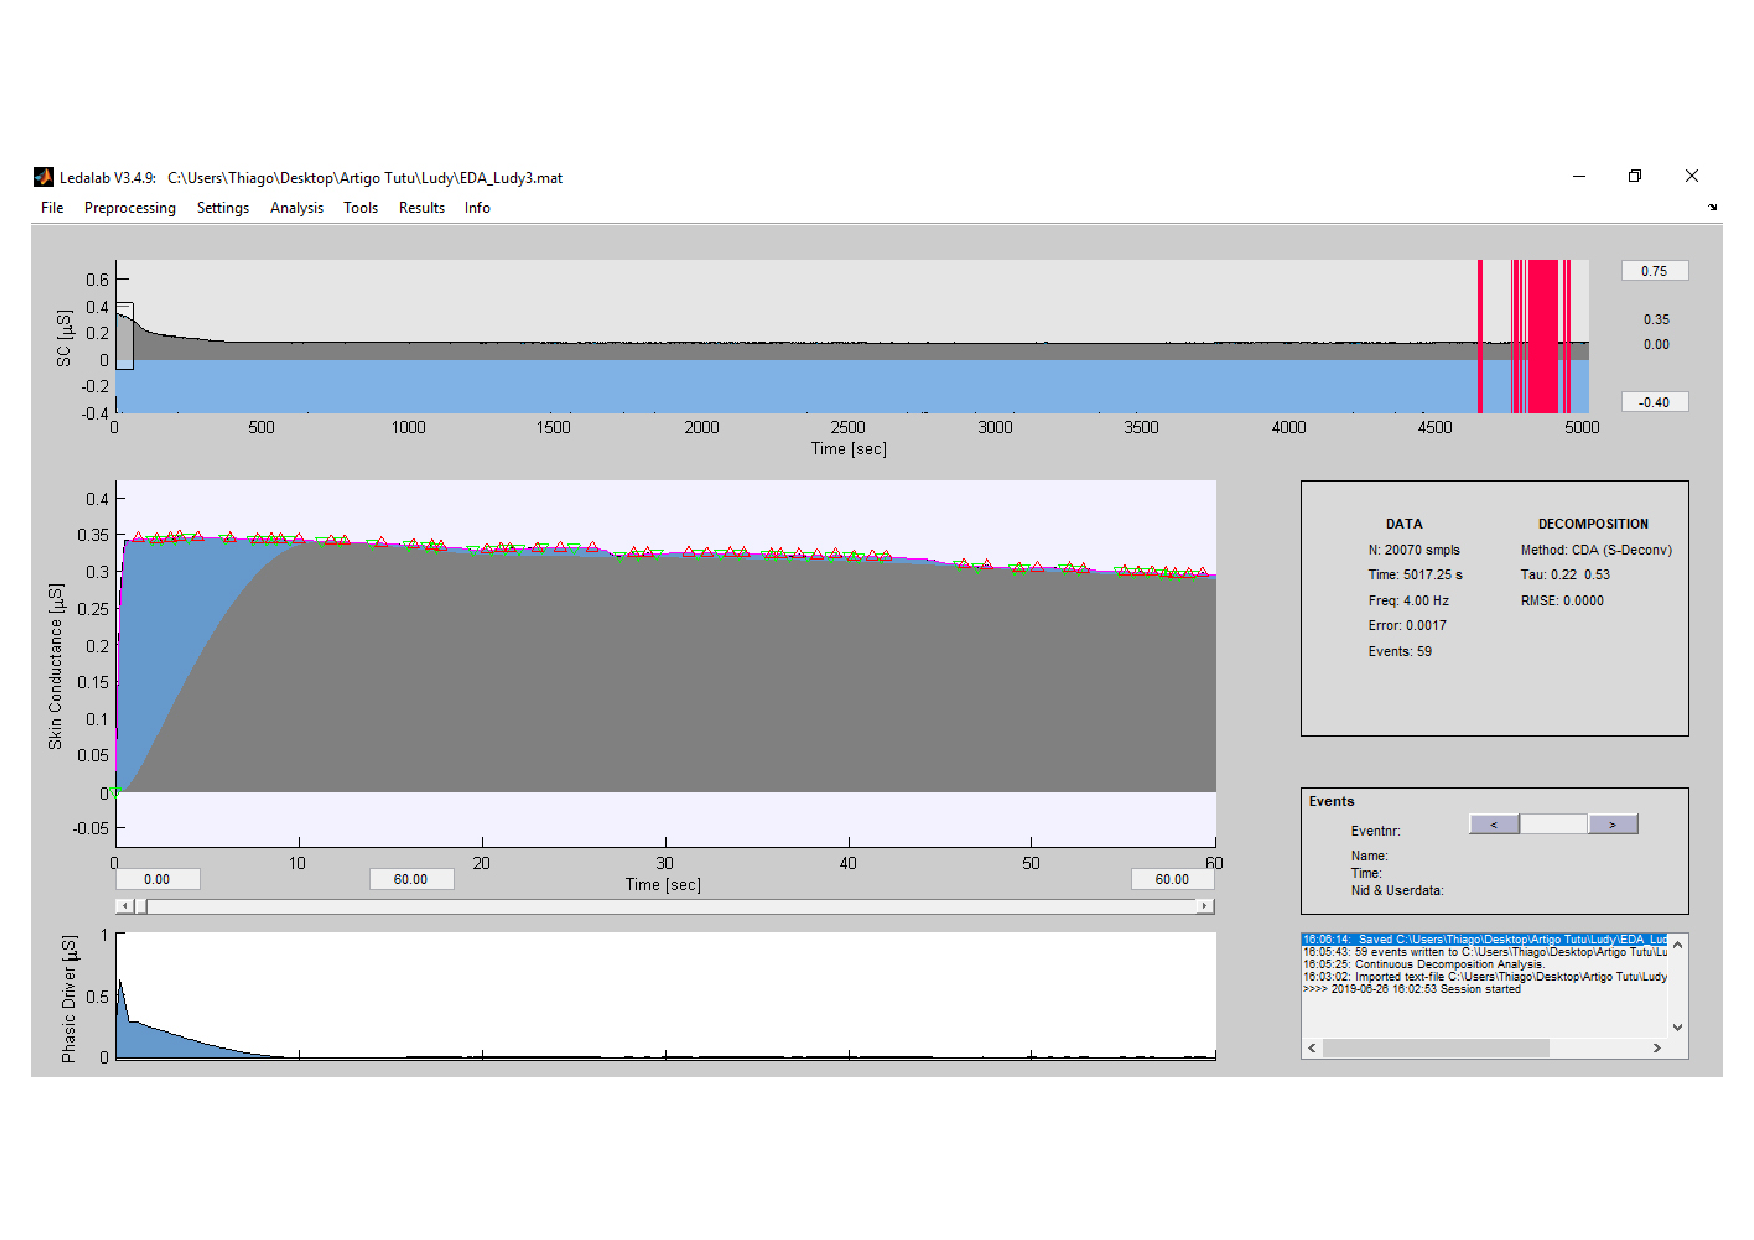
\includegraphics[width=1\linewidth]{img/cap4/ledalab}
\caption{Ledalab software used for EDA decomposition} \label{fig:ledalab}
\end{center}
\end{figure}

For evaluation of the event related skin conductance responses (each command given by the users is considered an event in this preliminary study), the phasic component is used, considering an event response window starting 1s after each event and finishing 4s after this same event \cite{khalfa2002}. The Continuous Decomposition Analysis (CDA) method is used, given its robustness on decomposing  EDA biosignals in continuous tonic and phasic data \cite{benedek2010}.

Amongst output variables extracted from Ledalab to evaluate individuals responses, the Integrated Skin Conductance Response (ISCR) is used. This metric consists of the time integral of the phasic driver extracted by Ledalab within the response window (1s to 4s after event). This variable is chosen since it considers both magnitude and duration of responses (it’s a time integral), while other available variables (count of SCRs, average SCR, sum of amplitudes of SCRs, SCR Phasic Max Response) take into account more unidimensional aspects of the responses. All data is standardized using z score shown in Equation (\ref{eq:zscore}) to reduce subject variability.

\begin{equation}\label{eq:zscore}
Z_{i} = \frac{X_{i}-\overline{X}}{S}
\end{equation}

Data processing of BVP is performed using Kubios, as shown in Figure \ref{fig:kubios}, a software used to analyze Heart Rate Variability (HRV)\cite{kubios2017, e4recom2020}. It utilizes Inter Beat Interval (IBI), extracted from BVP measured by the E4 wristband \cite{ibidata2020} for each user on each protocol. It returns several output variables, among them the Stress Index (SI) calculated as the square root of Baevsky's stress index \cite{baevsky2008}.

\begin{figure}[!hbt]
\begin{center}
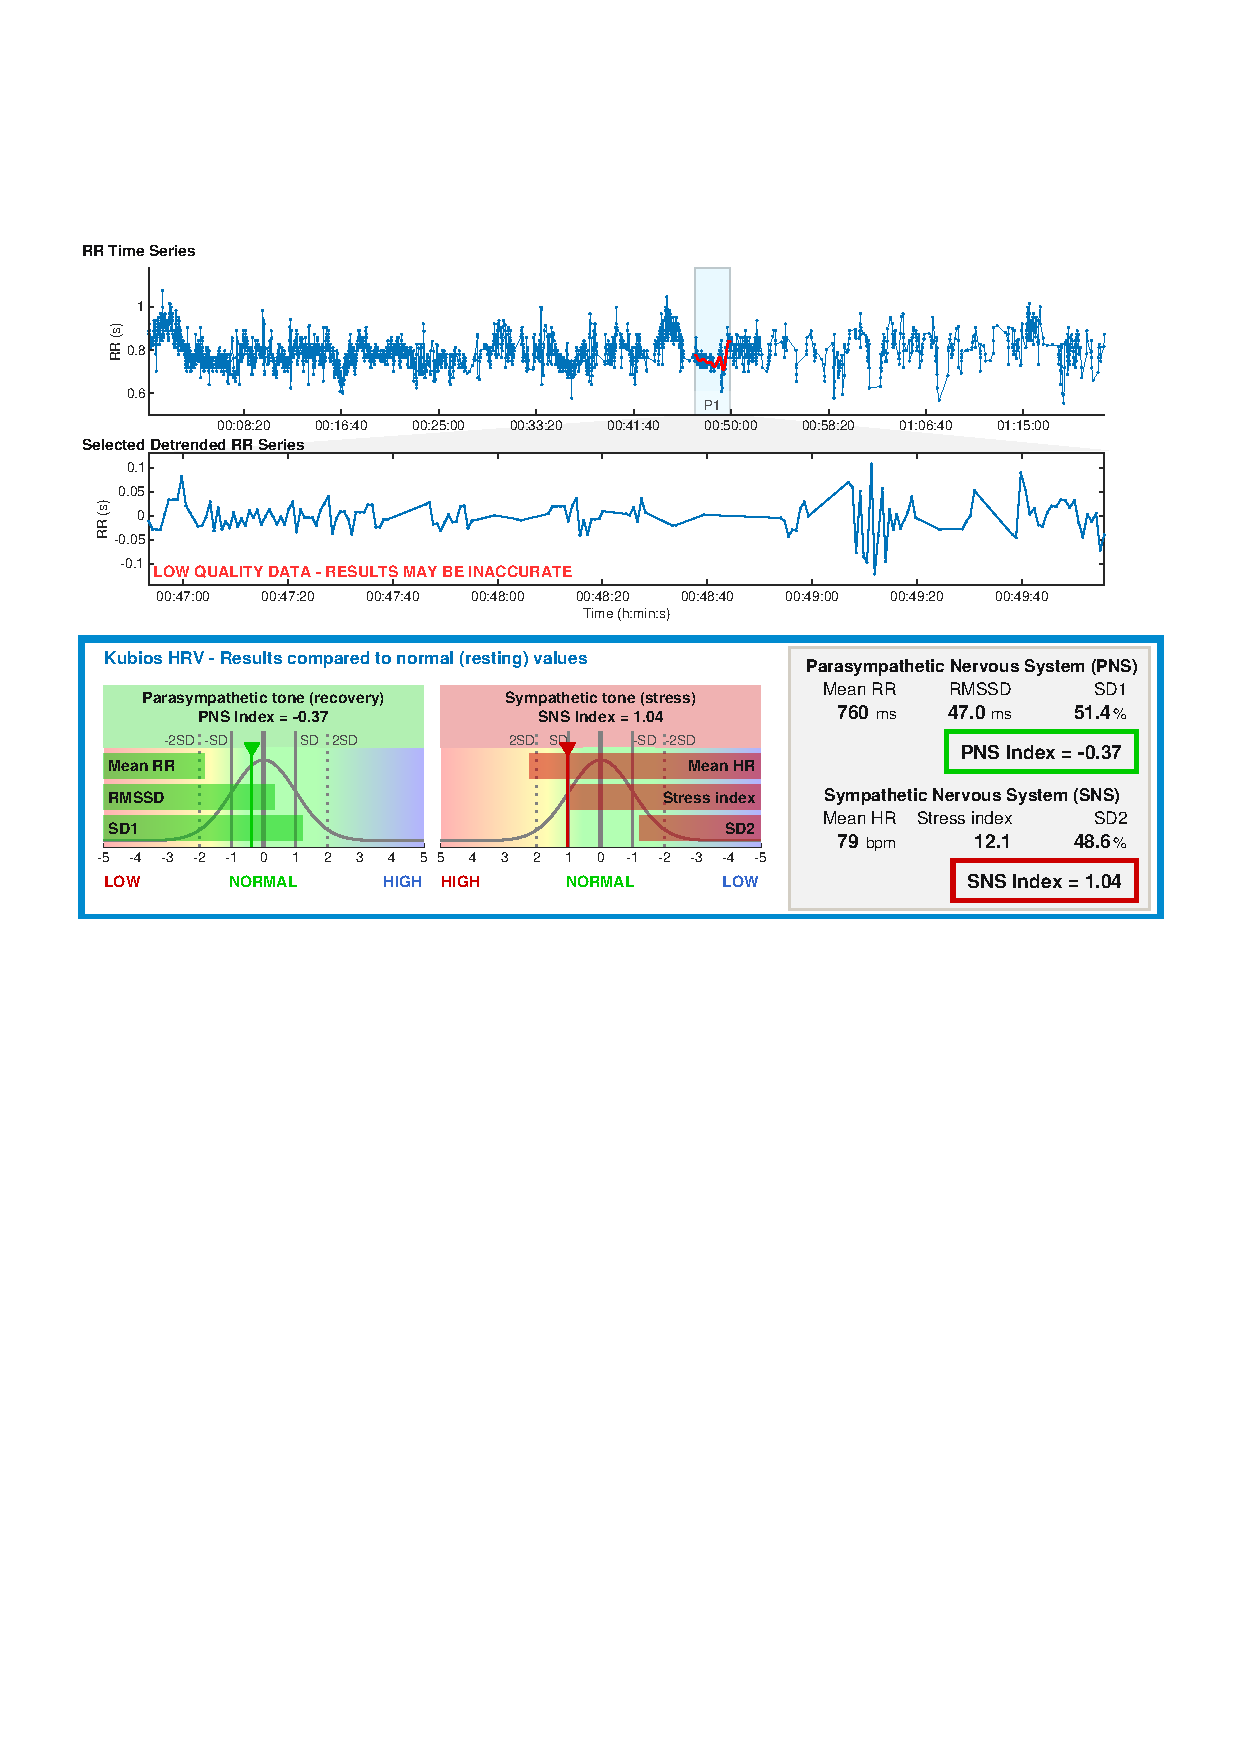
\includegraphics[width=1\linewidth]{img/cap4/kubios}
\caption{A section of a report generated by the Kubios software for HRV} \label{fig:kubios}
\end{center}
\end{figure}

\subsection{Assessment methodology}
\label{sec:assessmethod}

PMRT  was chosen by having a higher ICC value as describe in Section \ref{sec:pmrtICC} \cite{kamaraj2016}.  Different metrics help to track users' evolution during the training protocols and can be used to better grade tasks values that's range (1-4)  \cite{massengale2005}. Thus, parameters present on the first line of Table \ref{table:tbDataCollec} are adopted as training metrics. Also, the biosignals on the third line in Table \ref{table:tbDataCollec} are collected to give clues of the emotional state of the user during training protocol \cite{affanni2018}.

Table  \ref{table:tbDataAnaly} showns data analysis details coming from the user training experiment.

\begin{table}[!hbt]
\caption{Data analysis information}\label{table:tbDataAnaly}
\centering
\begin{tabular}{ >{\centering}m{0.5cm}  >{}m{14.5cm} }
\toprule
N.o &  Description \\
\midrule
1  	& The PMRT Methodology is used for trials performance evaluation;  \\ \midrule
2 	& Bar charts shown the users questions evaluation and Word clouds \cite{bletzer2015} represent the most relevant reasons for the user’s evaluations based on users and therapist’s comments/notes and; \\ \midrule
3 	& Protocols data analysis were divided in:
\begin{enumerate}
\item EDA Analysis, using ISCR as variable for statistical analysis between protocols. All statistical evaluations were made using the R-software$\texttrademark$ \cite{jurevckova2019}. The Shapiro-Wilk test is used, and the data distribution is found to be non-normal \cite{islam2019};
\item Stress Index Analysis, using the IBI time series (Inter-Beat Interval - Time between individual heart beats) is used to obtain the Stress Index for each protocol individually using the software Kubios \cite{hrvKubios2018}.
\end{enumerate} \\
\bottomrule
\end{tabular}
\end{table}


\section{Preliminary tests}
General information about volunteers in this research is shown in Table \ref{table:tbUserGeneral}.


\begin{table}[!htb]
\caption{Volunteers general information}\label{table:tbUserGeneral}
\centering
\begin{tabular}{ >{\centering}m{0.5cm}  >{}m{3.5cm}  >{}m{10.8cm} }
\toprule
No. & Description & Detail \\
\midrule
1 & Volunteers  	& Consist of 3 adults aged 22 to 57 years;  \\
2 & Gender 		& 1 woman and 2 men with spinal cord injury \cite{rizzo2019, nunnerley2017}; \\
3 & Location 		& Collection was made in a rehabilitation center 10 kilometers far from the training site; \\
4 & Consent form 	& Volunteers were asked to fill a consent form (Appendix III); \\
5 & Ethical Committee 	& The approval to conduct this research was obtained from the Federal University (377566140.0000.5152). \\
\bottomrule
\end{tabular}
\end{table}

Clinical information about the volunteers in this research is detailed in Table \ref{table:tbUserClinical}.

\begin{table}[!htb]
\caption{\label{table:tbUserClinical}Volunteers clinical information}
\centering
\begin{tabular}{ >{\centering}m{0.5cm}  >{}m{14.7cm} }
\toprule
N.o &  Detail \\
\midrule
1 	& He has 2 years of injury, has 18 months of experience in driving the Ottobock PW, drove a car previously, the user performance is satisfactory, the performance of ADL (feeding) / AIVD (change of posture, transport), has transportation (not adapted), house adapted to move around and needs joystick adaptation; \\ \midrule
2 	& He has 5 year of injury, has 48 months of experience in driving the Ortobrás PW, drove a car previously, the user performance is satisfactory, the performance of ADL (Dress, undress, put on.) / AIVD is semi independent, has adapted transportation, house fully adapted and requested a joystick position adaptation; \\ \midrule
3  	& She has 3 years of injury, has 6 months of experience in driving the Freedom PW, did not drive cars previously, the user performance is satisfactory but uses adaptation in the trachea, the ADL / AIVD performance  is semi independent and semi independent, it does not have transport, have significant spasms that affect postural control and PW control performance. She is not well positioned in the PW. Required posture revision and joystick adjustment.  \\ 
\bottomrule
\end{tabular}
\end{table}

\subsection{Procedure and process}
\label{sec:procedureProcess}
The initial process steps followed for each volunteer every first time, instructed and supported by a therapist, is described in Tables \ref{table:tbProcedure01} and \ref{table:tbProcedure02}.

\begin{table}[!hbt]
\caption{Procedure and Processes - Part 01}\label{table:tbProcedure01}
\centering
\begin{tabular}{ >{\centering}m{0.5cm}  >{}m{14.5cm} }
\toprule
Step & Procedure/Process \\
\midrule
1  &  Ensure that the environment temperature is conditioned at 25$^{\circ}$C for good quality of biosignals \cite{lanata2014};  \\ \cline{2-2}
2  &  Volunteers will be registered into the system by the therapist as a patient. Volunteers had the project explained again for purposes of clarification and for a chance to withdraw the study; \\ \cline{2-2}
3  &  Volunteers will be instructed about how to log into the system; \\ \cline{2-2}
4  &  Volunteers will be instructed about system functionalities and how to make the download of the application, responsible for transmitting the joystick commands to control the PW remotely; \\ \cline{2-2}
5  &  The remote environment will be presented for the volunteers in 360$^{\circ}$ and explained how he/she must proceed to interact with it; \\ \cline{2-2}
6  &  Volunteers will be instructed about how to request a training session; \\ \cline{2-2}
7  &  Let the volunteer rest for 7 minutes before starting each training session to ensure a good emotional state and relax \cite{lanata2014}; \\ \cline{2-2}
8  &  Wearing the ``E4 wristband'' wearable device as shown in Figure \ref{fig:e4wristband}; \\ \cline{2-2}
9 &  Request the training sessions. \\ 
\bottomrule
\end{tabular}
\end{table}

\begin{table}[!hbt]
\caption{Procedure and Processes - Part 02}\label{table:tbProcedure02}
\centering
\begin{tabular}{ >{\centering}m{0.5cm}  >{}m{14.5cm} }
\toprule
Step & Procedure/Process \\
\midrule
10 &  While the therapist is selecting one of the preliminaries training protocols which are: drive straight forward (4.5 meters) in a narrow corridor without hitting the walls; turning right and left 90$^{\circ}$ and maneuver the chair by an access ramp, the volunteer reads all information about how to proceed in front of each virtual object; \\ \cline{2-2}
11 &  At the end of each protocol, volunteers are invited to fill out a survey questionnaire with advantages, disadvantages and suggestions or observations about the protocol performed, while the therapist is evaluating the trial performed;  \\ \cline{2-2}
12 &  Volunteers have to rest for 5 minutes between each training session to ensure comfort and absence of side effects before another request \cite{lanata2014}; \\ \cline{2-2}
13 &  After the last protocol, volunteers are invited to fill out other questions related to his/her own individual profile and system requisites; \\ \cline{2-2}
14 &  The study ended. \\ 
\bottomrule
\end{tabular}
\end{table}

The survey questionnaires are shown in Tables \ref{table:tbSurvey01} and \ref{table:tbSurvey02}. They were built based on the observations coming from Valentini et al. \cite{valentini2019},  Borresen et al. \cite{borresen2019}, Kamaraj et al. \cite{kamaraj2016}  which aboard users individual profiles and system requisites. In order for the volunteer can be able to better express the intensity of their perception for each question, we choose to use the Likert scale \cite{likert1932}. The volunteer can express his opinion by indicating one of the options on a five-point scale. Normaly, the values vary from 1 to 5, or 5 to 1, or even from -2 to 2, but always representing five different intensities of agreement or disagreement.

\begin{table}[!hbt]
\caption{Survey Questionaire - Part 01}\label{table:tbSurvey01}
\centering
\begin{tabular}{ >{\centering}m{0.5cm}   >{\centering}m{2.5cm}   >{\centering}m{2.5cm}   >{\centering}m{2.5cm}  >{\centering}m{2.5cm}   >{\centering}m{2.8cm} }
\toprule
N.o                                    & \multicolumn{5}{l}{Question Asked}                                                                                                                                 \\ \midrule
\multicolumn{1}{c}{\multirow{3}{*}{1}} & \multicolumn{5}{l}{How was to learn about using the system?}                                                                                                           \\
\multicolumn{1}{c}{}                   & \multicolumn{1}{c}{5}         & \multicolumn{1}{c}{4}    & \multicolumn{1}{c}{3}               & \multicolumn{1}{c}{2}         & \multicolumn{1}{c}{1}              \\
\multicolumn{1}{c}{}                   & \multicolumn{1}{>{\centering}m{2.5cm}}{Very Easy} & \multicolumn{1}{>{\centering}m{2.5cm}}{Easy} & \multicolumn{1}{>{\centering}m{2.5cm}}{Relatively Easy} & \multicolumn{1}{>{\centering}m{2.5cm}}{Difficult} & \multicolumn{1}{>{\centering}m{2.8cm}}{Very Difficult} \\ \cline{2-6}

\multicolumn{1}{c}{\multirow{3}{*}{2}} & \multicolumn{5}{l}{How do you evaluate the graphical interface of the system?}                                                                                                           \\
\multicolumn{1}{c}{}                   & \multicolumn{1}{c}{5}         & \multicolumn{1}{c}{4}    & \multicolumn{1}{c}{3}               & \multicolumn{1}{c}{2}         & \multicolumn{1}{c}{1}              \\
\multicolumn{1}{c}{}                   & \multicolumn{1}{>{\centering}m{2.5cm}}{Great} & \multicolumn{1}{>{\centering}m{2.5cm}}{Very good} & \multicolumn{1}{>{\centering}m{2.5cm}}{Good} & \multicolumn{1}{>{\centering}m{2.5cm}}{Median} & \multicolumn{1}{>{\centering}m{2.8cm}}{Bad} \\ \cline{2-6}
\multicolumn{1}{c}{\multirow{3}{*}{3}} & \multicolumn{5}{l}{How was it to use the system?}                                                                                                           \\
\multicolumn{1}{c}{}                   & \multicolumn{1}{c}{5}         & \multicolumn{1}{c}{4}    & \multicolumn{1}{c}{3}               & \multicolumn{1}{c}{2}         & \multicolumn{1}{c}{1}              \\
\multicolumn{1}{c}{}                   & \multicolumn{1}{>{\centering}m{2.5cm}}{Very easy} & \multicolumn{1}{>{\centering}m{2.5cm}}{Easy} & \multicolumn{1}{>{\centering}m{2.5cm}}{Relatively easy} & \multicolumn{1}{>{\centering}m{2.5cm}}{Difficult} & \multicolumn{1}{>{\centering}m{2.8cm}}{Very difficult} \\ \cline{2-6} 
\multicolumn{1}{c}{\multirow{3}{*}{4}} & \multicolumn{5}{l}{Did the system meet the navigation needs?}                                                                                                           \\
\multicolumn{1}{c}{}                   & \multicolumn{1}{c}{5}         & \multicolumn{1}{c}{4}    & \multicolumn{1}{c}{3}               & \multicolumn{1}{c}{2}         & \multicolumn{1}{c}{1}              \\
\multicolumn{1}{c}{}                   & \multicolumn{1}{>{\centering}m{2.5cm}}{Excellent} & \multicolumn{1}{>{\centering}m{2.5cm}}{Great} & \multicolumn{1}{>{\centering}m{2.5cm}}{Good} & \multicolumn{1}{>{\centering}m{2.5cm}}{Median} & \multicolumn{1}{>{\centering}m{2.8cm}}{Bad} \\        
\bottomrule
\end{tabular}
\vspace{20pt}
\end{table}

\begin{table}[!hbt]
\caption{Survey Questionaire - Part 02}\label{table:tbSurvey02}
\centering
\begin{tabular}{ >{\centering}m{0.3cm}   >{\centering}m{1.2cm}   >{\centering}m{1.2cm}   >{\centering}m{1.2cm}  >{\centering}m{1.2cm}   >{\centering}m{1.2cm} }
\toprule
N.o                                    & \multicolumn{5}{l}{Question Asked}                                                                                                                                 \\ \midrule
\multicolumn{1}{c}{\multirow{3}{*}{5}} & \multicolumn{5}{l}{How do you consider the quality of the image presented?}                                                                                                           \\
\multicolumn{1}{c}{}                   & \multicolumn{1}{c}{5}         & \multicolumn{1}{c}{4}    & \multicolumn{1}{c}{3}               & \multicolumn{1}{c}{2}         & \multicolumn{1}{c}{1}              \\
\multicolumn{1}{c}{}                   & \multicolumn{1}{>{\centering}m{2.5cm}}{Excelent} & \multicolumn{1}{>{\centering}m{2.5cm}}{Great} & \multicolumn{1}{>{\centering}m{2.5cm}}{Good} & \multicolumn{1}{>{\centering}m{2.5cm}}{Median} & \multicolumn{1}{>{\centering}m{2.8cm}}{Bad} \\  \cline{2-6}


\multicolumn{1}{c}{\multirow{3}{*}{6}} & \multicolumn{5}{l}{Do you consider that the AR (virtual objects) help to carry out the training?}                                                                                                           \\
\multicolumn{1}{c}{}                   & \multicolumn{1}{c}{5}         & \multicolumn{1}{c}{4}    & \multicolumn{1}{c}{3}               & \multicolumn{1}{c}{2}         & \multicolumn{1}{c}{1}              \\
\multicolumn{1}{c}{}                   & \multicolumn{1}{>{\centering}m{2.5cm}}{Very} & \multicolumn{1}{>{\centering}m{2.5cm}}{Moderate} & \multicolumn{1}{>{\centering}m{2.5cm}}{Medium} & \multicolumn{1}{>{\centering}m{2.5cm}}{Little} & \multicolumn{1}{>{\centering}m{2.8cm}}{None} \\  \cline{2-6}

\multicolumn{1}{c}{\multirow{3}{*}{7}} & \multicolumn{5}{l}{How was the processing time (response time)?}                                                                                                           \\
\multicolumn{1}{c}{}                   & \multicolumn{1}{c}{5}         & \multicolumn{1}{c}{4}    & \multicolumn{1}{c}{3}               & \multicolumn{1}{c}{2}         & \multicolumn{1}{c}{1}              \\
\multicolumn{1}{c}{}                   & \multicolumn{1}{>{\centering}m{2.5cm}}{Very fast} & \multicolumn{1}{>{\centering}m{2.5cm}}{Fast} & \multicolumn{1}{>{\centering}m{2.5cm}}{Moderate} & \multicolumn{1}{>{\centering}m{2.5cm}}{Slow} & \multicolumn{1}{>{\centering}m{2.8cm}}{Very slow} \\ \cline{2-6} 


\multicolumn{1}{c}{\multirow{3}{*}{8}} & \multicolumn{5}{l}{How much do you consider this tool assists in the development of driving skills?}                                                                                                           \\
\multicolumn{1}{c}{}                   & \multicolumn{1}{c}{5}         & \multicolumn{1}{c}{4}    & \multicolumn{1}{c}{3}               & \multicolumn{1}{c}{2}         & \multicolumn{1}{c}{1}              \\
\multicolumn{1}{c}{}                   & \multicolumn{1}{>{\centering}m{2.5cm}}{Intensily} & \multicolumn{1}{>{\centering}m{2.5cm}}{Very} & \multicolumn{1}{>{\centering}m{2.5cm}}{Moderately} & \multicolumn{1}{>{\centering}m{2.5cm}}{Little} & \multicolumn{1}{>{\centering}m{2.8cm}}{Nothing} \\ \cline{2-6}

\multicolumn{1}{c}{\multirow{3}{*}{9}} & \multicolumn{5}{l}{How do you evaluate your well-being after training?}                                                                                                           \\
\multicolumn{1}{c}{}                   & \multicolumn{1}{c}{5}         & \multicolumn{1}{c}{4}    & \multicolumn{1}{c}{3}               & \multicolumn{1}{c}{2}         & \multicolumn{1}{c}{1}              \\
\multicolumn{1}{c}{}                   & \multicolumn{1}{>{\centering}m{2.5cm}}{Relaxed} & \multicolumn{1}{>{\centering}m{2.5cm}}{Little tired} & \multicolumn{1}{>{\centering}m{2.5cm}}{Tired} & \multicolumn{1}{>{\centering}m{2.5cm}}{Very tired} & \multicolumn{1}{>{\centering}m{2.8cm}}{Exhausted} \\  \cline{2-6}

\multicolumn{1}{c}{\multirow{3}{*}{10}} & \multicolumn{5}{l}{Are you satisfied with the system features?}                                                                                                           \\
\multicolumn{1}{c}{}                   & \multicolumn{1}{c}{5}         & \multicolumn{1}{c}{4}    & \multicolumn{1}{c}{3}               & \multicolumn{1}{c}{2}         & \multicolumn{1}{c}{1}              \\
\multicolumn{1}{c}{}                   & \multicolumn{1}{>{\centering}m{2.5cm}}{Very Satisfied} & \multicolumn{1}{>{\centering}m{2.5cm}}{Satisfied} & \multicolumn{1}{>{\centering}m{2.5cm}}{Indifferent} & \multicolumn{1}{>{\centering}m{2.5cm}}{Dissatisfied} & \multicolumn{1}{>{\centering}m{2.8cm}}{Very dissatisfied} \\  \cline{2-6}

\multicolumn{1}{c}{\multirow{3}{*}{11}} & \multicolumn{5}{l}{Does the system do what it was meant to do?}                                                                                                           \\
\multicolumn{1}{c}{}                   & \multicolumn{1}{c}{5}         & \multicolumn{1}{c}{4}    & \multicolumn{1}{c}{3}               & \multicolumn{1}{c}{2}         & \multicolumn{1}{c}{1}              \\ 
\multicolumn{1}{c}{}                   & \multicolumn{1}{>{\centering}m{2.5cm}}{Extremely well} & \multicolumn{1}{>{\centering}m{2.5cm}}{Very well} & \multicolumn{1}{>{\centering}m{2.5cm}}{Well} & \multicolumn{1}{>{\centering}m{2.5cm}}{Relatively well} & \multicolumn{1}{>{\centering}m{2.8cm}}{Nothing} \\
\bottomrule
\end{tabular}
\end{table}

The next section presents the web server application requirements in detail.

\section{Web server application}
\label{sec:webserverApp}

The Java$\texttrademark$ Servlet technology provides consistent mechanism that makes possible the development  of an architecture with the following features: video streams, different channels to receive/redirect data, to generate data during user experience and system platform independency \cite{sun2003}.  The Model-View-Controller (MVC) is an architectural pattern that separates an application into three main logical components: the model, the view, and the controller \cite{basham2008}.

The web server application runs on client (patient and therapist) site, through the browser. Browsers such Google Chrome, Internet Explorer and Mozilla Firefox runs over a tightly controlled environment called sandbox \cite{quong2020,taivalsaari2008}. A sandbox application can restrict piece of running code when, for instance, a javascript or a browser extension, try to access local resources\footnote{Universal Serial Bus (USB) and High-Definition Multimedia Interface (HDMI)  devices or user data} \cite{quong2020}. It is only possible to access physical resources when the application is running locally. However, when the user needs to use the webcam for an example, he is requested to allow the use of this resource. It often happens, when is requested to establish a video stream connection using the WebRTC (Web Real-Time Communication) framework, implemented by the latest browsers affording multi-video-streaming channels between peers \cite{ha2020, edan2020, garcia2020}.

Most of the times, it is not possible to access data from control devices such eye tracker, Rift HMD and others, without a run time installation. Also, it is not possible to install this into a browser. Therefore, it is necessary to have a local app running on the patient site computer, to establish a data channel between patient site and web server.


Figure \ref{fig:mvc-layersArch} visualize all MVC components that come from the system architecture requirements and Use Cases (UC). The following sections, highlight the UML Sequence Diagram (UML-SD) that describes how each component's actions are connected.

\begin{figure}[!hbt]
\begin{center}
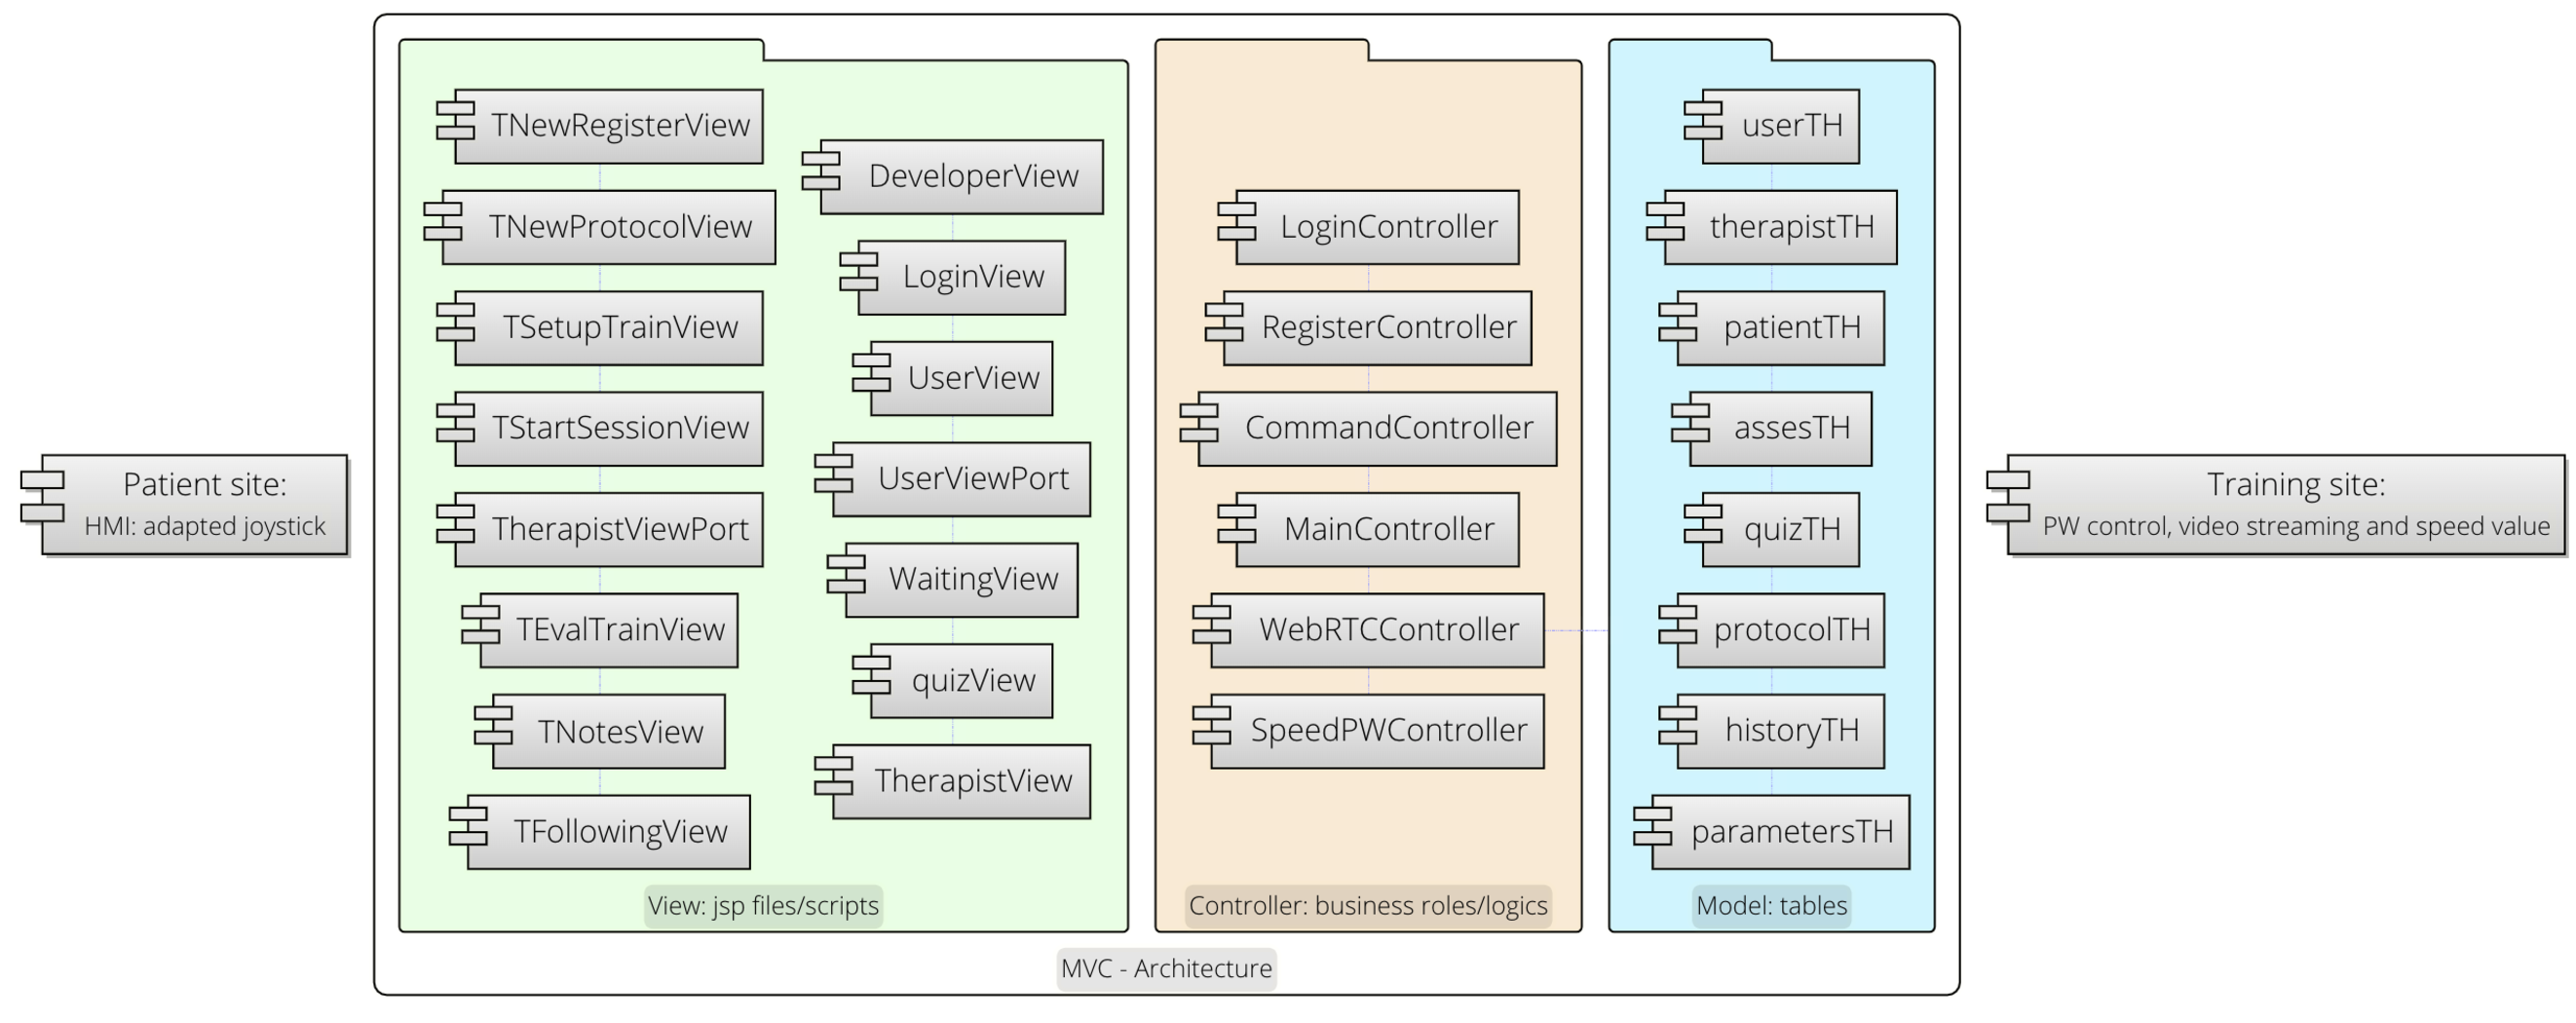
\includegraphics[width=1\linewidth]{img/cap4/mvc-layersArch}
\caption{MVC application components} \label{fig:mvc-layersArch}
\end{center}
\end{figure}

\subsection{Administrator: Parametrize system UML-SD}

Based on the administrador UC actions, defined on Figure \ref{fig:adminCase},  the administrator UML-SD is presented in Figure \ref{fig:UMLSD-Administrator}.


\begin{figure}[!hbt]
\begin{center}
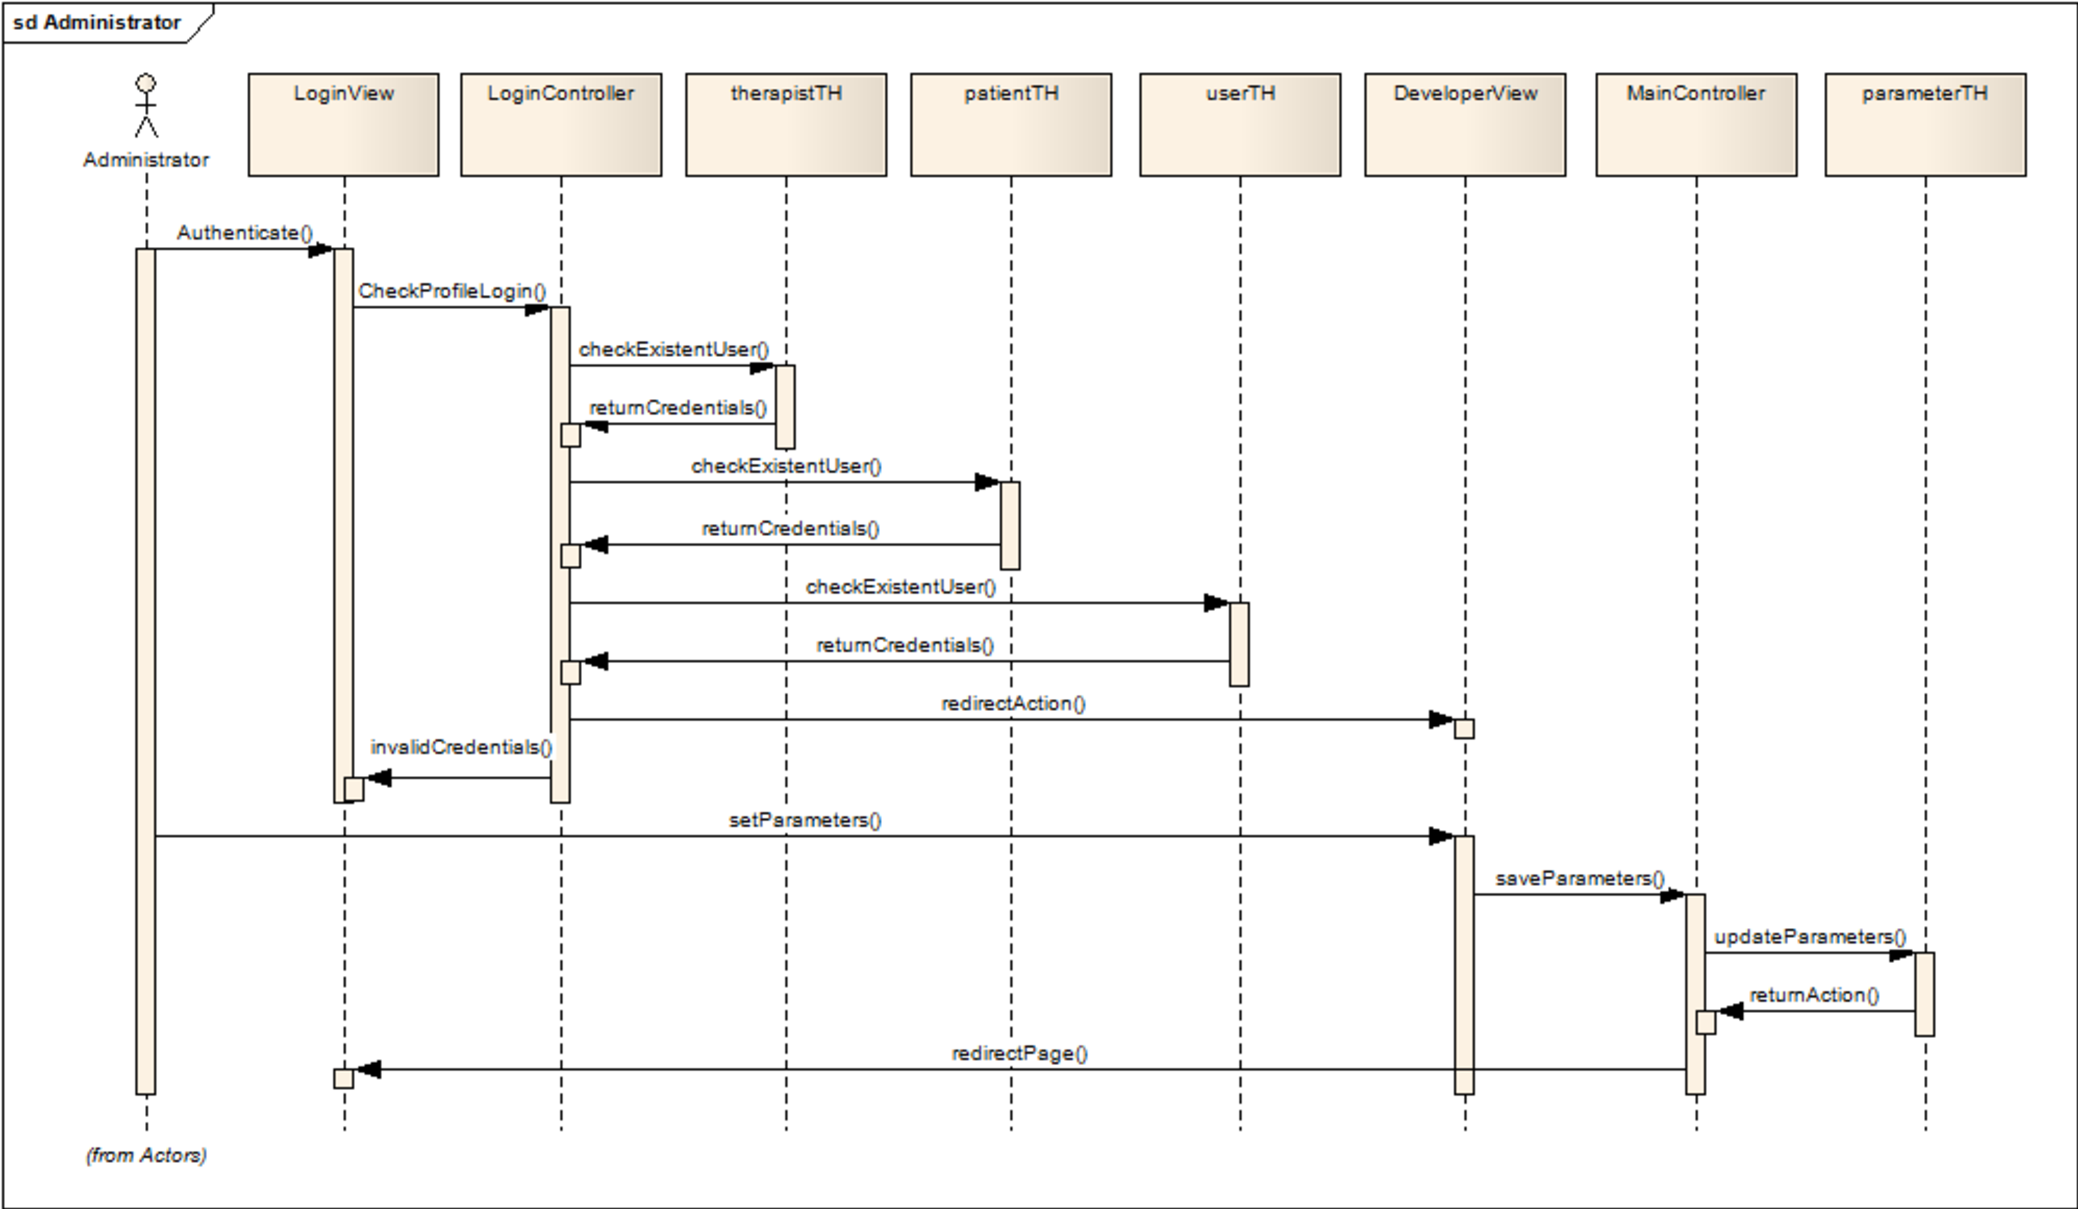
\includegraphics[width=1 \textwidth]{img/cap4/UMLSD-Administrator}
\caption{Administrator: Parametrize system UML-SD}
\label{fig:UMLSD-Administrator}
\end{center}
\end{figure} 

These actions are essencial because some systemic internal actions depend on this parameters such as the Internet Protocol Address (IP) of training site, the protocol used between each site, the IP of patient site and if at the end of training session the user have to fill the survey.


\subsection{User actions UML-SD}
\subsubsection{User local use case UML-SD}

Based on the user local UC actions, defined on Figure \ref{subfig:userCaseLocal},  the respective UML-SD is shown in Figure \ref{fig:UMLSD-UserLocalCase}.

\begin{figure}[!hbt]
\begin{center}
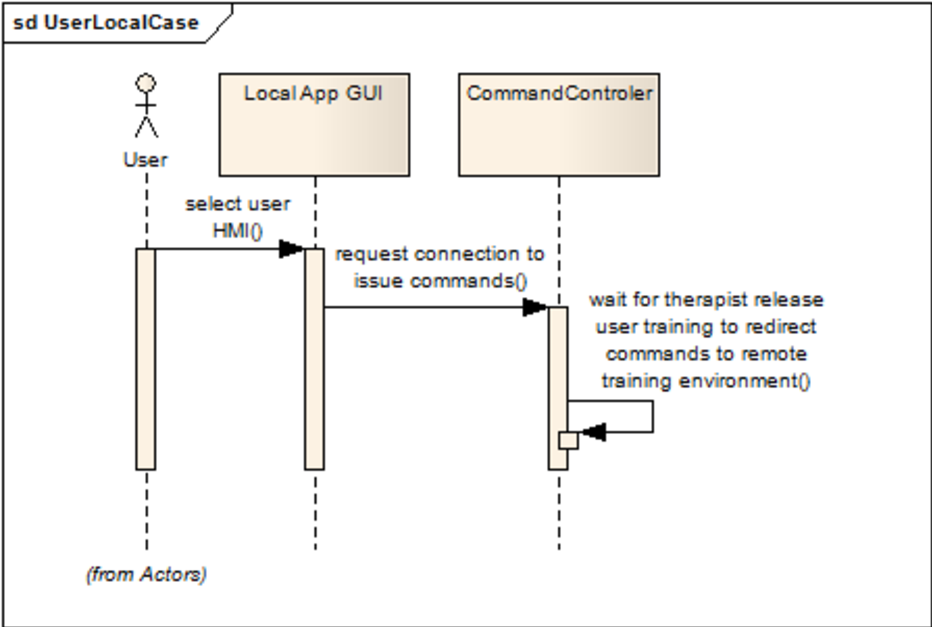
\includegraphics[width=0.5 \textwidth]{img/cap4/UMLSD-UserLocalCase}
\caption{Issuing commands locally  - User UML-SD}
\label{fig:UMLSD-UserLocalCase}
\end{center}
\end{figure} 

As a browser is considered a sandbox \cite{quong2020}, it is necessary to take in count the need for a cross-platform runtime app to allow the user to transmit the control commands to the webserver. While the therapist has not finalized the training settings, to be performed by the requesting user, no commands will be computed or redirected to the training environment.


\subsubsection{User Web use case UML-SD}

As presented in Figure \ref{fig:UMLSD-UserWebCase01}, the user have to proceed with the authentication in web application. Later, he/she is redirected to user ``UserView''. In this view, he/she must select the HMI to be used in agreement to his/her impairment and request his/her training. Until the therapist finish his tasks the user have to stay at ``WaitingView''.

\begin{figure}[!hbt]
\begin{center}
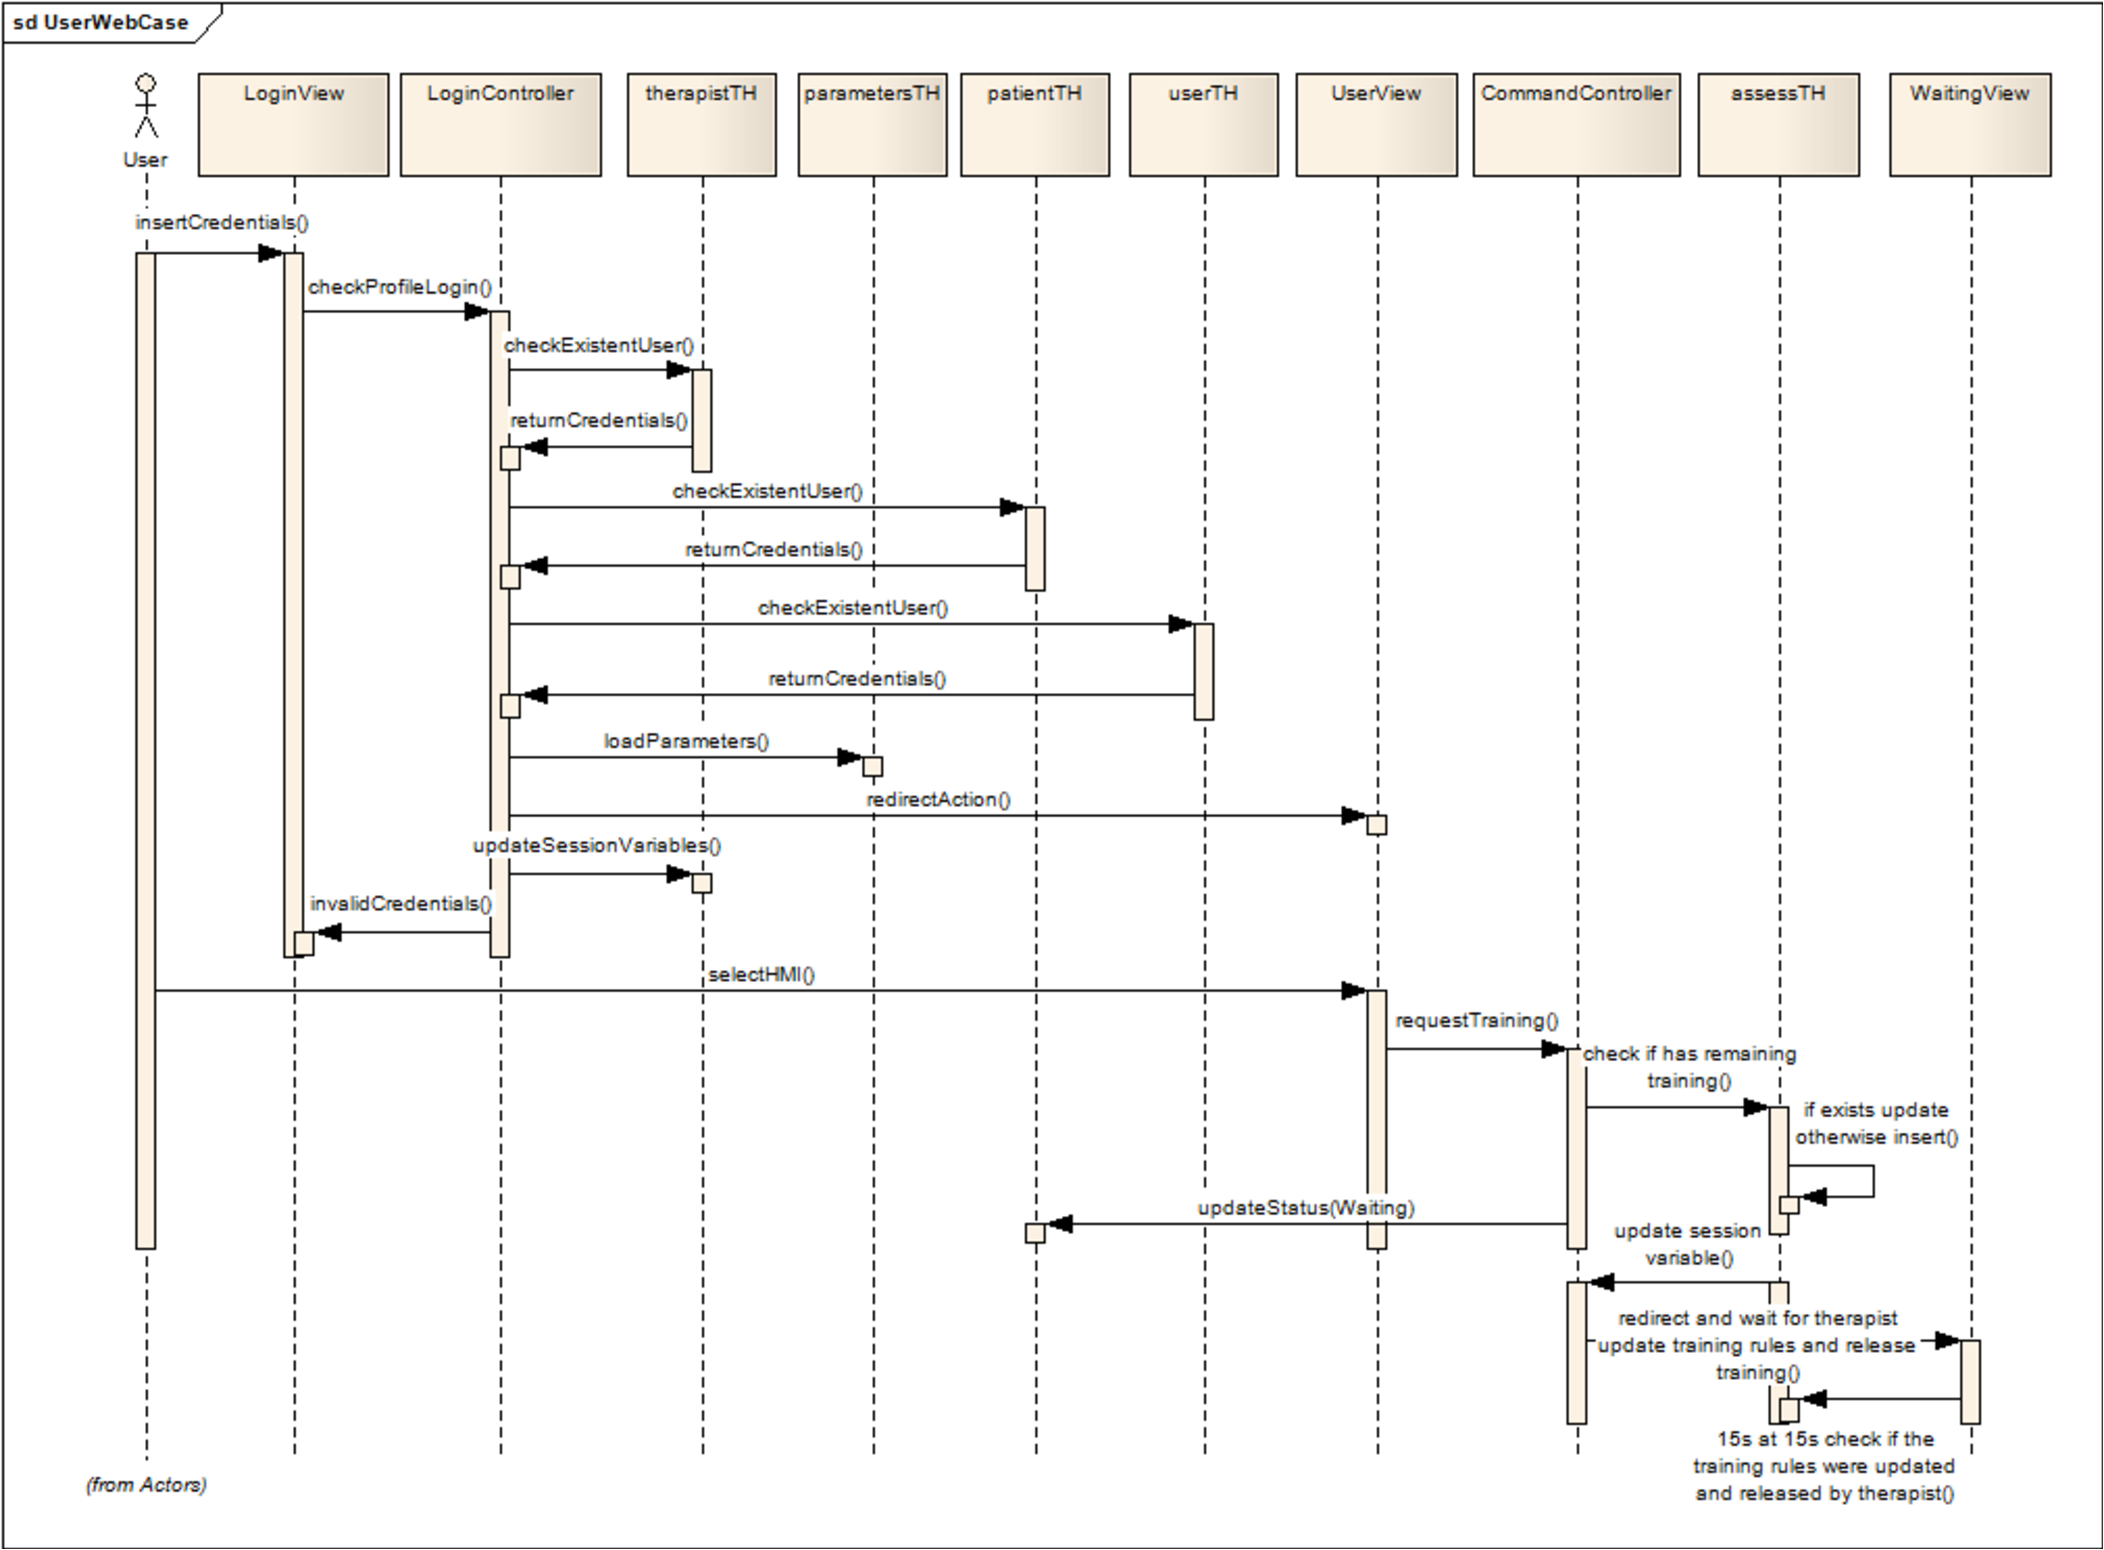
\includegraphics[width=1 \textwidth]{img/cap4/UMLSD-UserWebCase01}
\caption{Web authentication and request training part one - User UML-SD}
\label{fig:UMLSD-UserWebCase01}
\end{center}
\end{figure} 

Figure \ref{fig:UMLSD-UserWebCase02} continues with the UML-SD. After the therapist had setup the user training protocol and started a video streaming from mobile device at training environment, the respective data are update to the table and them the user is redirected to ``UserViewPort''. Where his/her command will be redirected to remote training site and preview augmented visual feedback. By finishing the training session, the user will be redirected to the survey page where he/she will invited to fill out all the information, presented in Table \ref{table:tbProcedure02} line 11 and all questions from Tables \ref{table:tbSurvey01} and \ref{table:tbSurvey02}.



\begin{figure}[!hbt]
\begin{center}
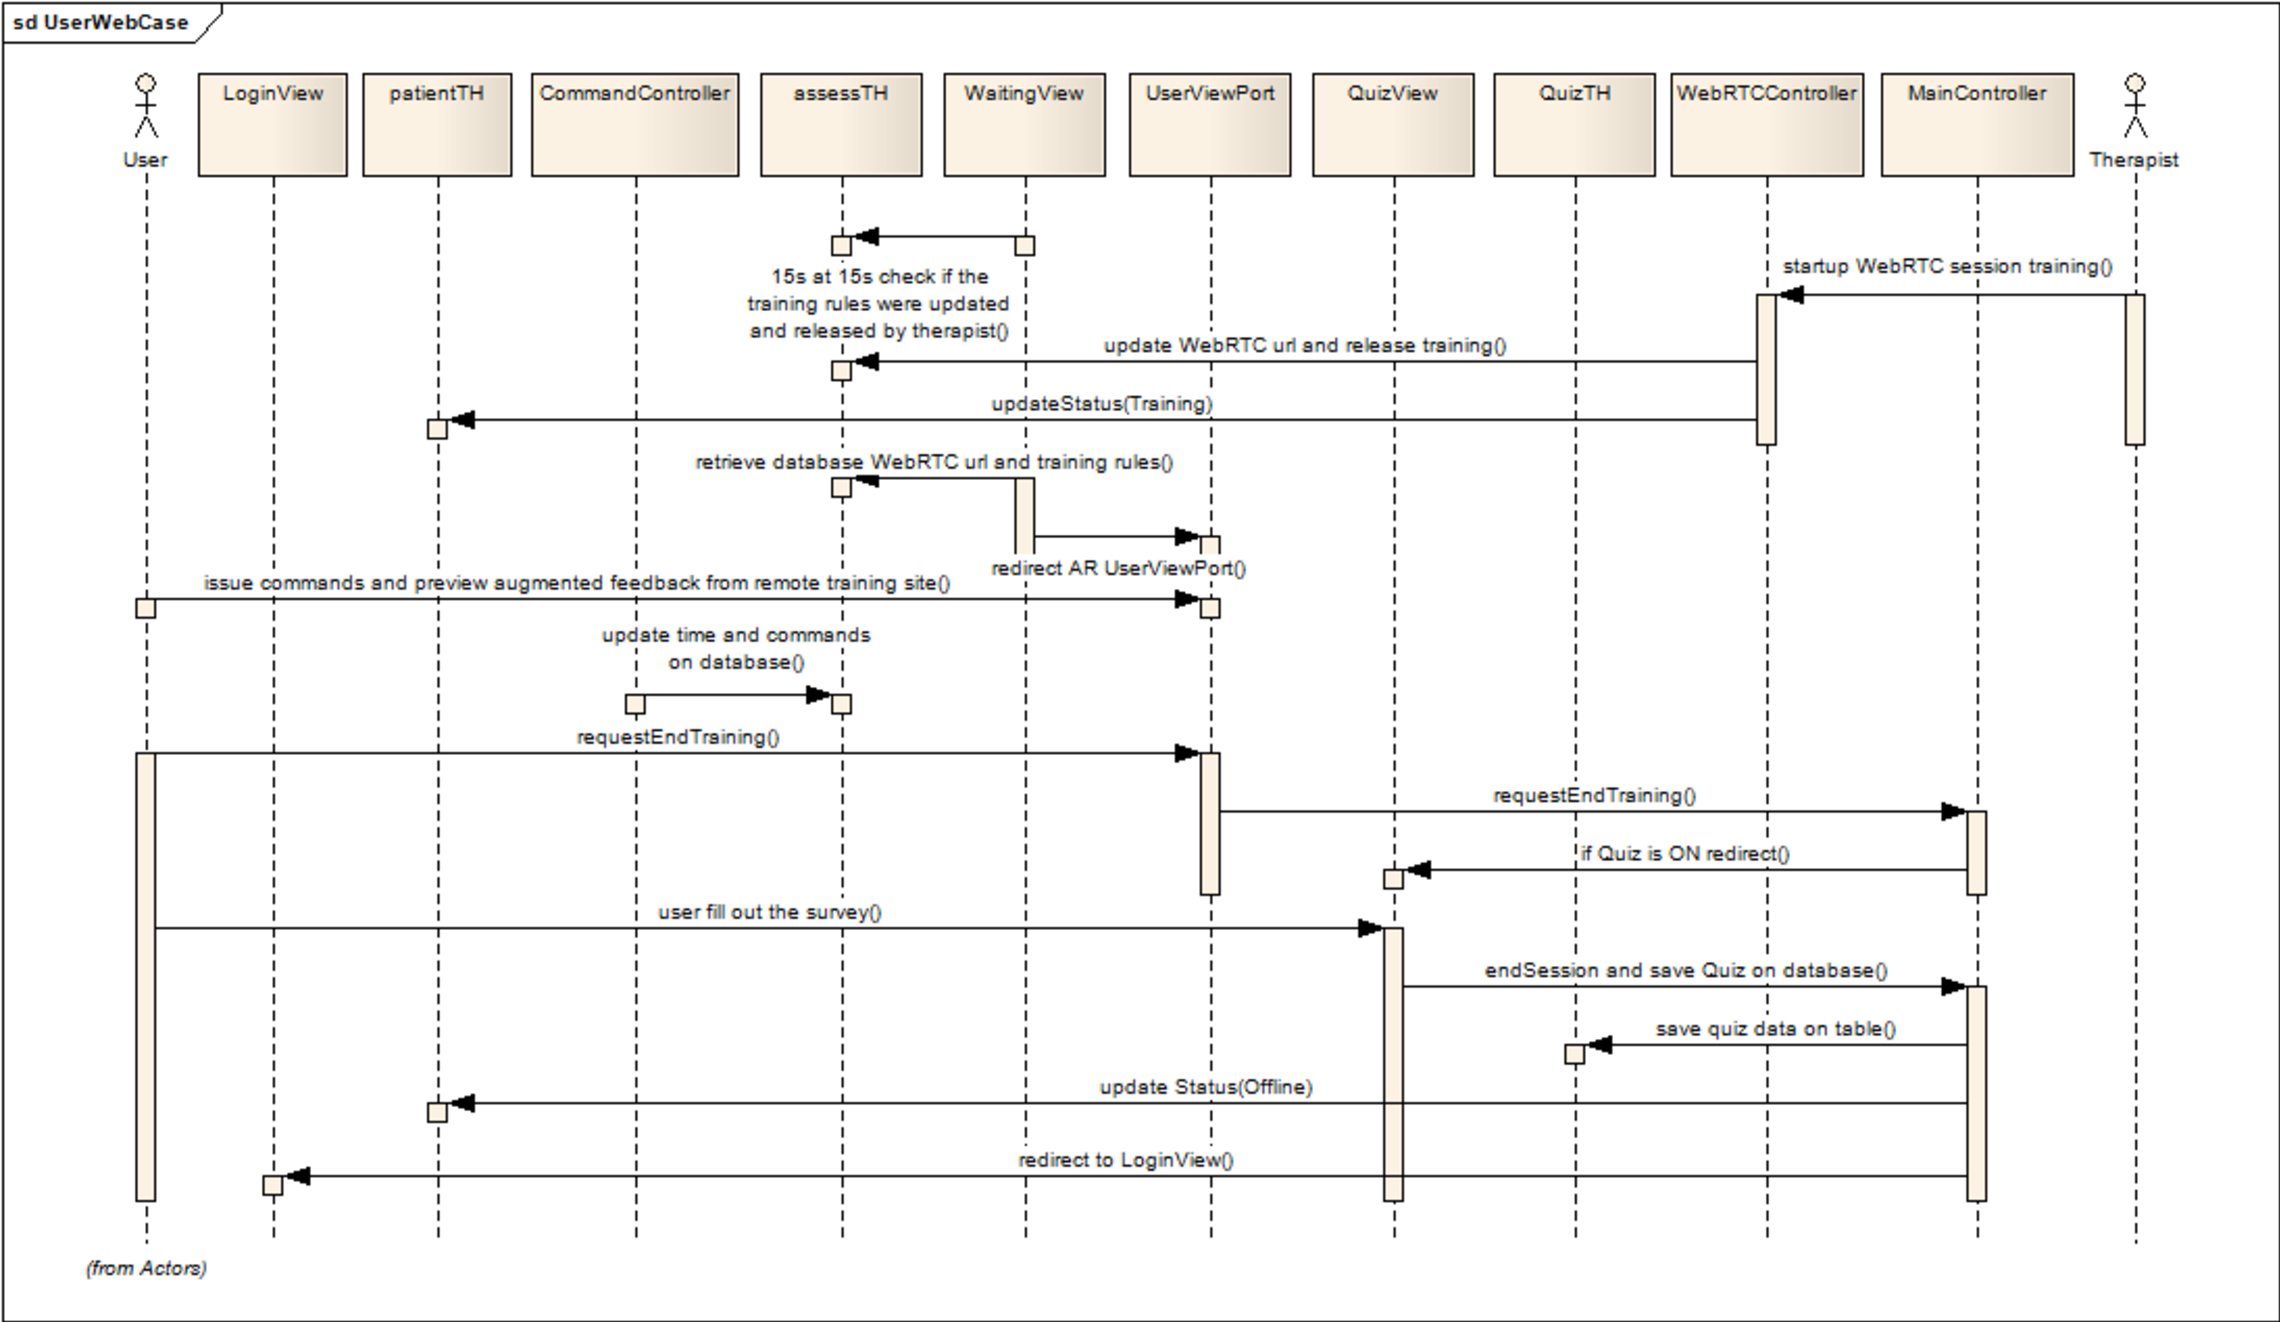
\includegraphics[width=1 \textwidth]{img/cap4/UMLSD-UserWebCase02}
\caption{Web perform training proposed and fill the quiz part two - User UML-SD}
\label{fig:UMLSD-UserWebCase02}
\end{center}
\end{figure} 


\subsection{Therapist action use case diagrams}
\subsubsection{Therapist authentication Web use case UML-SD}

As presented in Figure \ref{fig:UMLSD-TherapistWebCase01}, the therapist have to proceed with the authentication in web application. Later, he is redirected to therapist ``TherapistView''. In this view, therapist have access to all actions inherited on the UC shown in Figure \ref{fig:therapistCases}.

\begin{figure}[!hbt]
\begin{center}
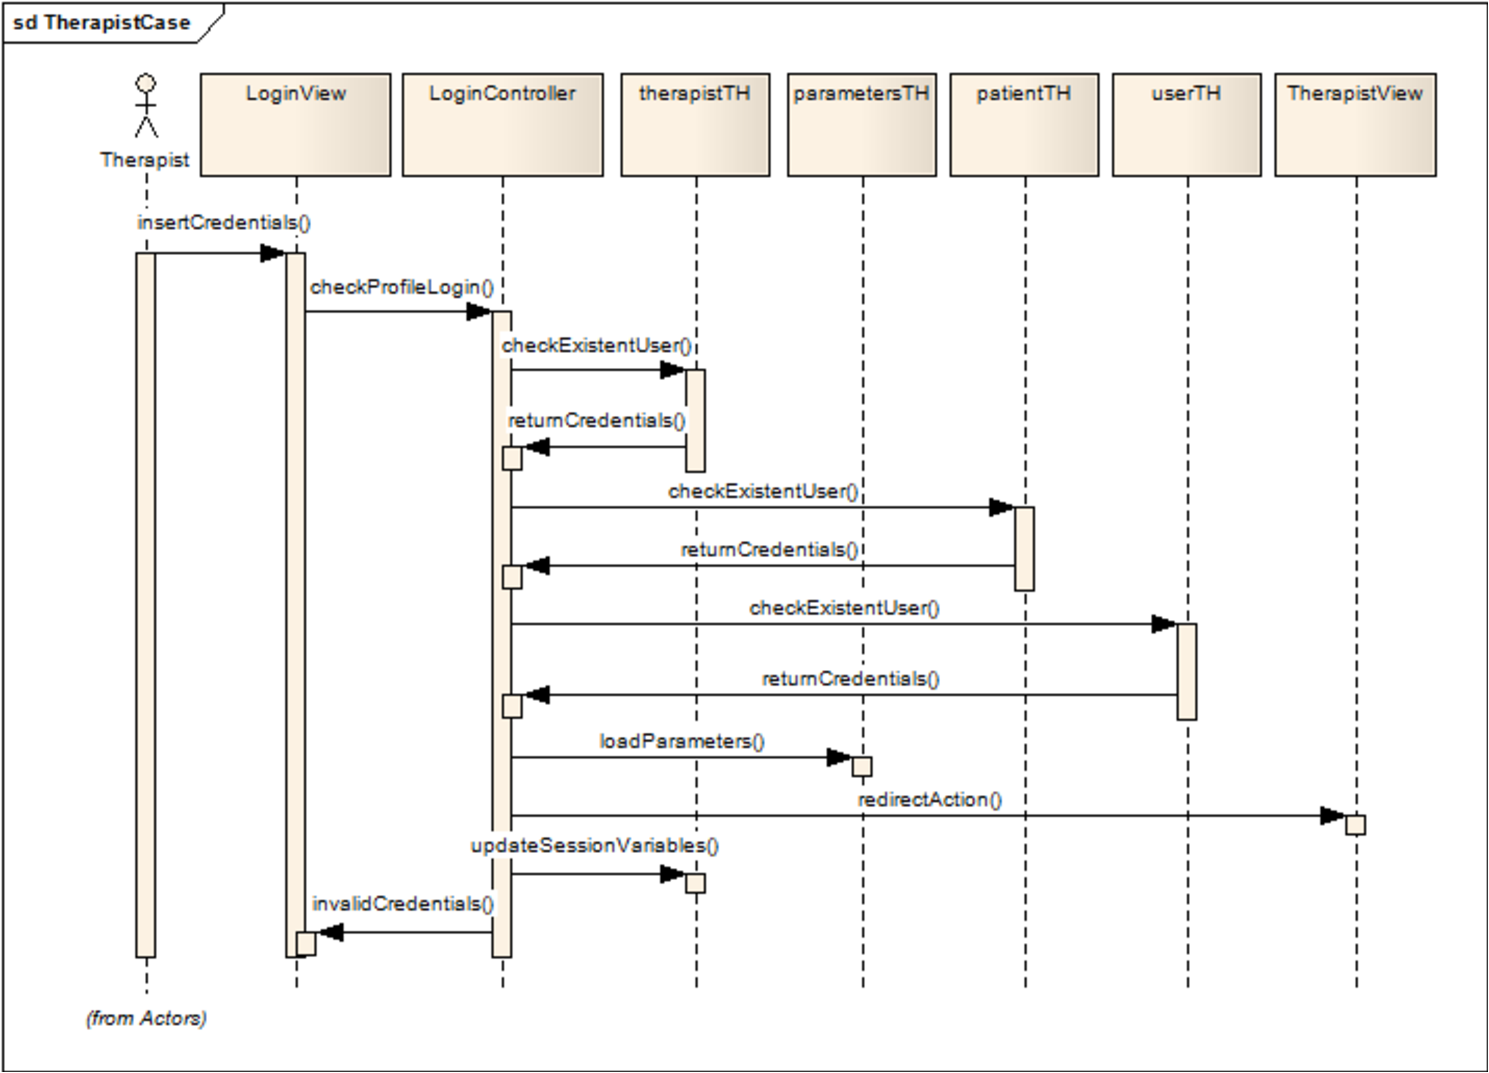
\includegraphics[width=0.71 \textwidth]{img/cap4/UMLSD-TherapistWebCase01}
\caption{Web authentication - Therapist UML-SD}
\label{fig:UMLSD-TherapistWebCase01}
\end{center}
\end{figure} 

\subsubsection{Therapist register new user Web use case UML-SD}

As presented in Figure \ref{fig:UMLSD-TherapistWebCase02}, the therapist has to proceed with the new user registration, as stated in Figure \ref{fig:therapistCases}. In the ``TherapistView'', he can access the ``TNewRegisterView'' and he may insert a new user considering two profiles: Therapist or Patient. 

\begin{figure}[!hbt]
\begin{center}
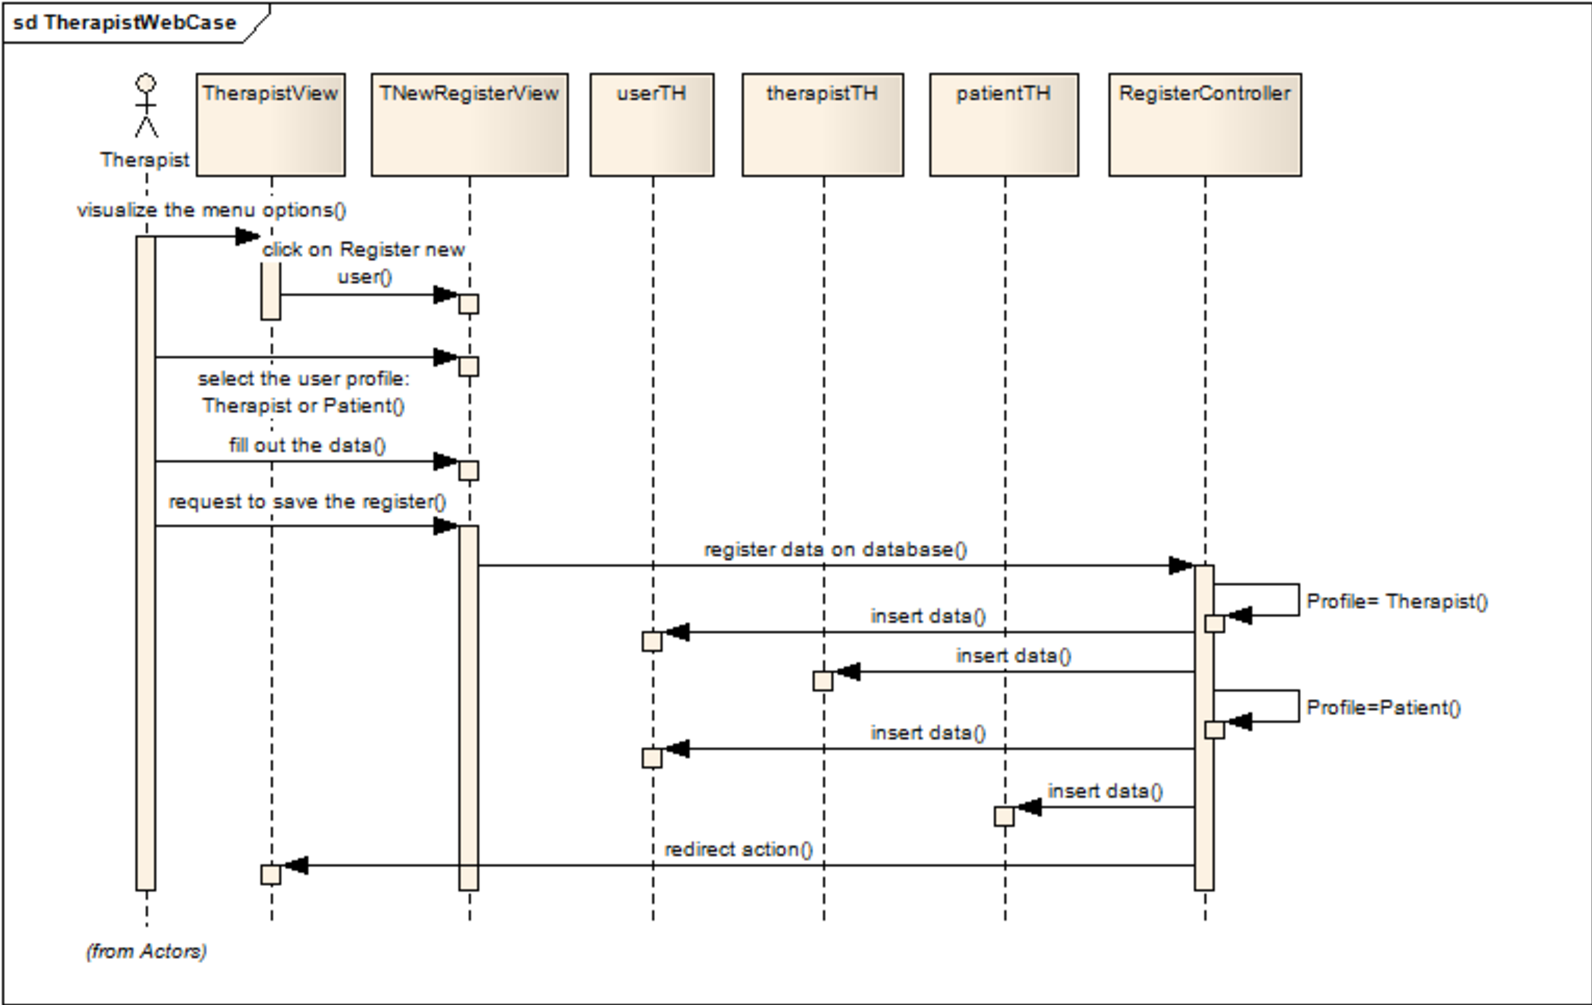
\includegraphics[width=0.7 \textwidth]{img/cap4/UMLSD-TherapistWebCase02}
\caption{Web register new user - Therapist UML-SD}
\label{fig:UMLSD-TherapistWebCase02}
\end{center}
\vspace{-20pt}
\end{figure} 

\subsubsection{Therapist new protocol Web use case UML-SD}

As presented in Figure \ref{fig:UMLSD-TherapistWebCase03}, the therapist has to proceed with the new protocol creation, as stated in Figure \ref{fig:therapistCases}. 

\begin{figure}[!hbt]
\begin{center}
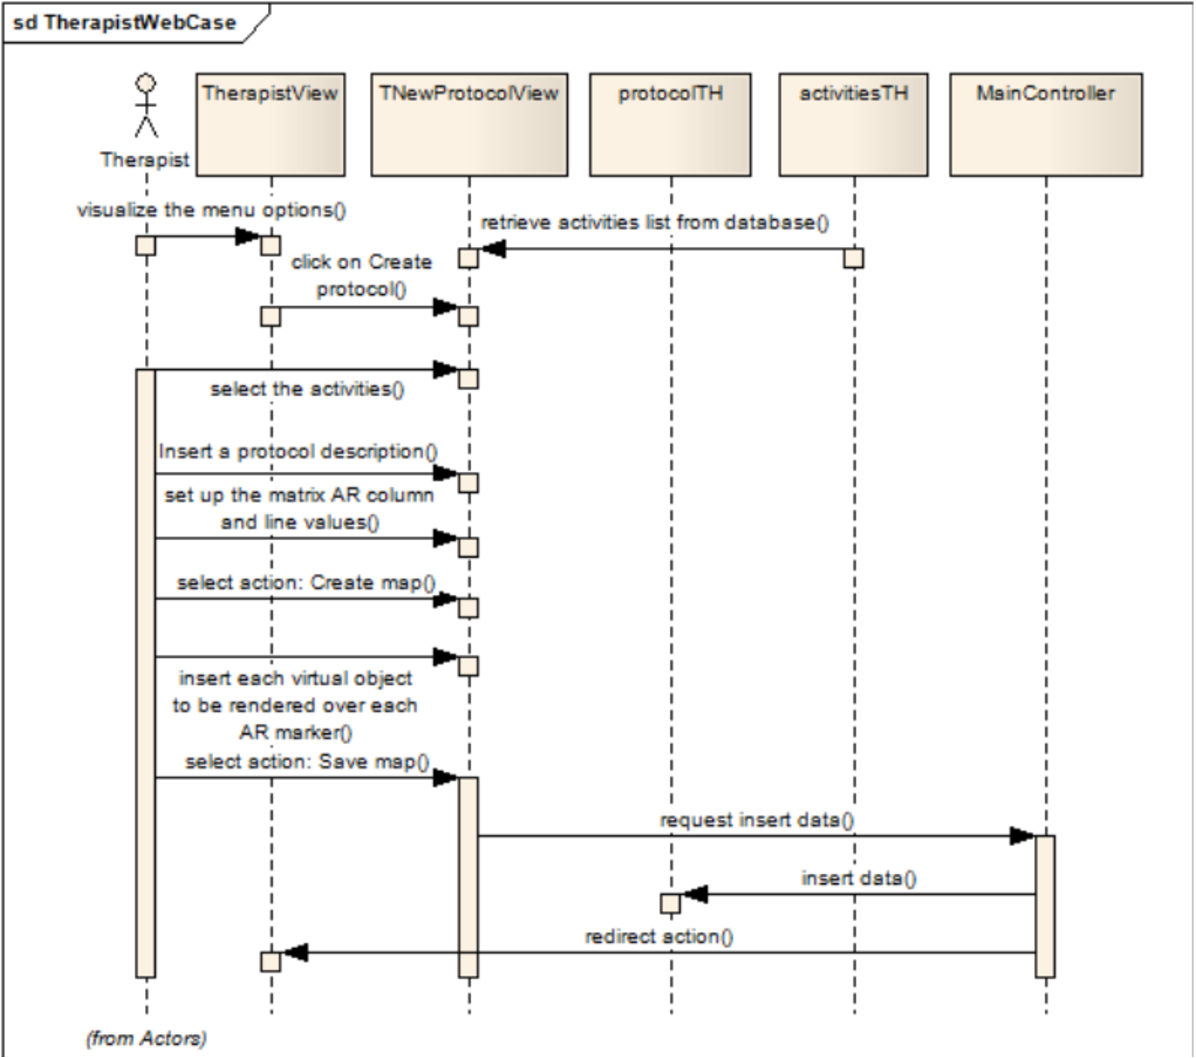
\includegraphics[width=0.65 \textwidth]{img/cap4/UMLSD-TherapistWebCase03}
\caption{Web create new protocol - Therapist UML-SD}
\label{fig:UMLSD-TherapistWebCase03}
\end{center}
\end{figure} 

In the ``TherapistView'', he can access the ``TNewProtocolView'' and he may create a new protocol. The following actions may be performed in order to accomplish the protocol creation:

\begin{enumerate}[label=(\alph*)]
\item Select the activity list that compounds the protocols' tasks. Taking in count the adaptations highlighted in Section \ref{sec:protocoTadaptation} and the 60 surveys filled out by the users, different activities of those that exist in PMRT might be used in the future;
\item Define a brief description of the protocol, for example, ``Protocol 01: detailed characteristics''. The special character ``:'' is used to split short name and protocol details;
\item Define the column number and line number of AR matrix used to create a new protocol training;
\item To created an empty AR map the ``Create map'' action was defined;
\item Select the virtual objects, among them must have ``static'' and ``animated'' object to guarantee the two main classes of activities of PMRT. These object might be used as a guidance, avoidance or with specifics actions;
\item To save the created protocol, the ``Save protocol'' action was defined;
\item To clear the map created, the ``Clear map'' action was defined; and
\item To end session, the ``Close'' action was defined.
\end{enumerate}

\subsubsection{Therapist define training use case UML-SD}

As presented in Figure \ref{fig:UMLSD-TherapistWebCase04}, the therapist has to define which action is performed for each training requisition. Among the action, until the user starts to train, are: ``Define protocol'', ``begin a session'' and ``follow the training'', shown in Figure \ref{fig:therapistCases}. From the ``TherapistView'', the menu option ``TSetupTrainView'' where the previous training requests can be previewed and accessed. 

\begin{figure}[!hbt]
\begin{center}
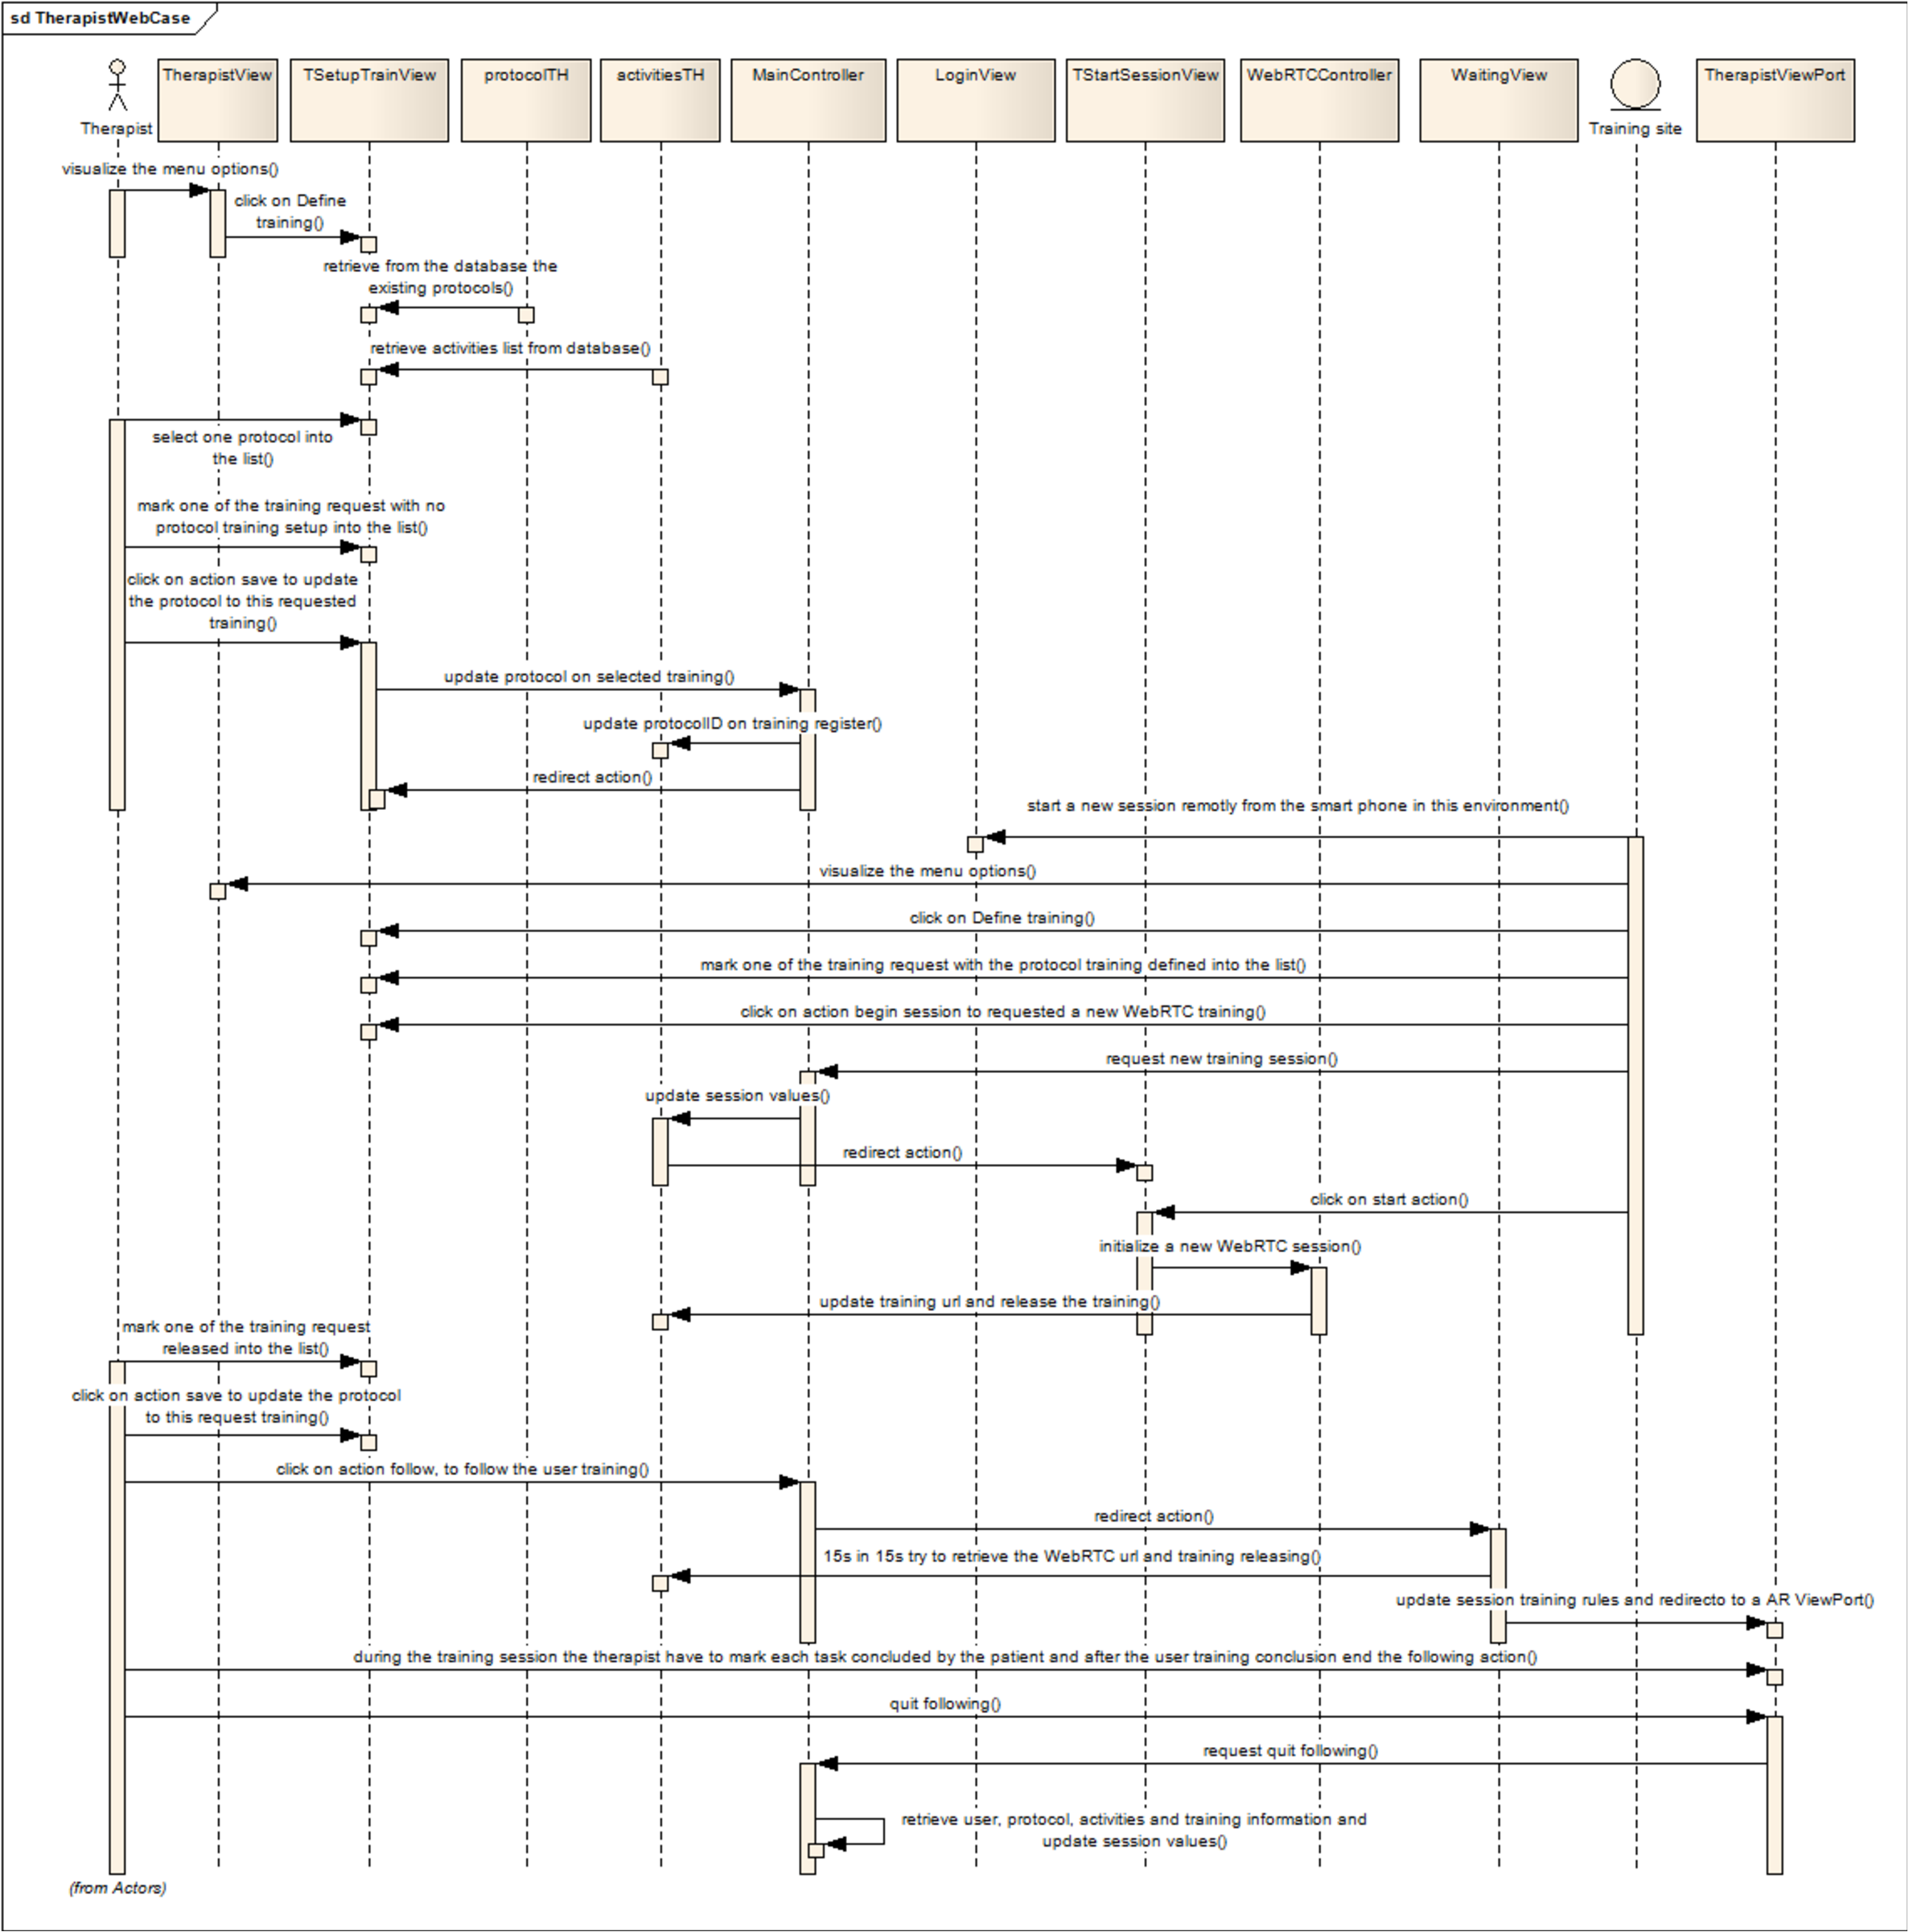
\includegraphics[width=1 \textwidth]{img/cap4/UMLSD-TherapistWebCase04}
\caption{Web define training view actions - Therapist UML-SD}
\label{fig:UMLSD-TherapistWebCase04}
\end{center}
\end{figure} 

To apply one of these actions, the therapist always has to select one training requirement before, selecting the action. It is only possible to begin a session to some training request that already has his/her protocol defined. It is only possible to follow the training of a request made, which the session was already initiated. 

When the ``begin session'' action is selected, the smartphone attached in PW, is remotely accessed to open a video streaming from the training site, where the AR markers and all physical components used to create a better training experience were placed. The pure video streaming (video and audio) is received in each site and augmented to the enrichment of the user experience. 

In the next section, the remaining actions triggered after the followed training are detailed.

\subsubsection{Therapist evaluate and note training use case UML-SD}

As presented in Figure \ref{fig:UMLSD-TherapistWebCase05}, the therapist is invited to evaluate the user training and take notes for each task into the protocol as defined in Figure \ref{fig:therapistCases}, following the considerations realized in Section \ref{sec:assessmethod}.  

\begin{figure}[!hbt]
\begin{center}
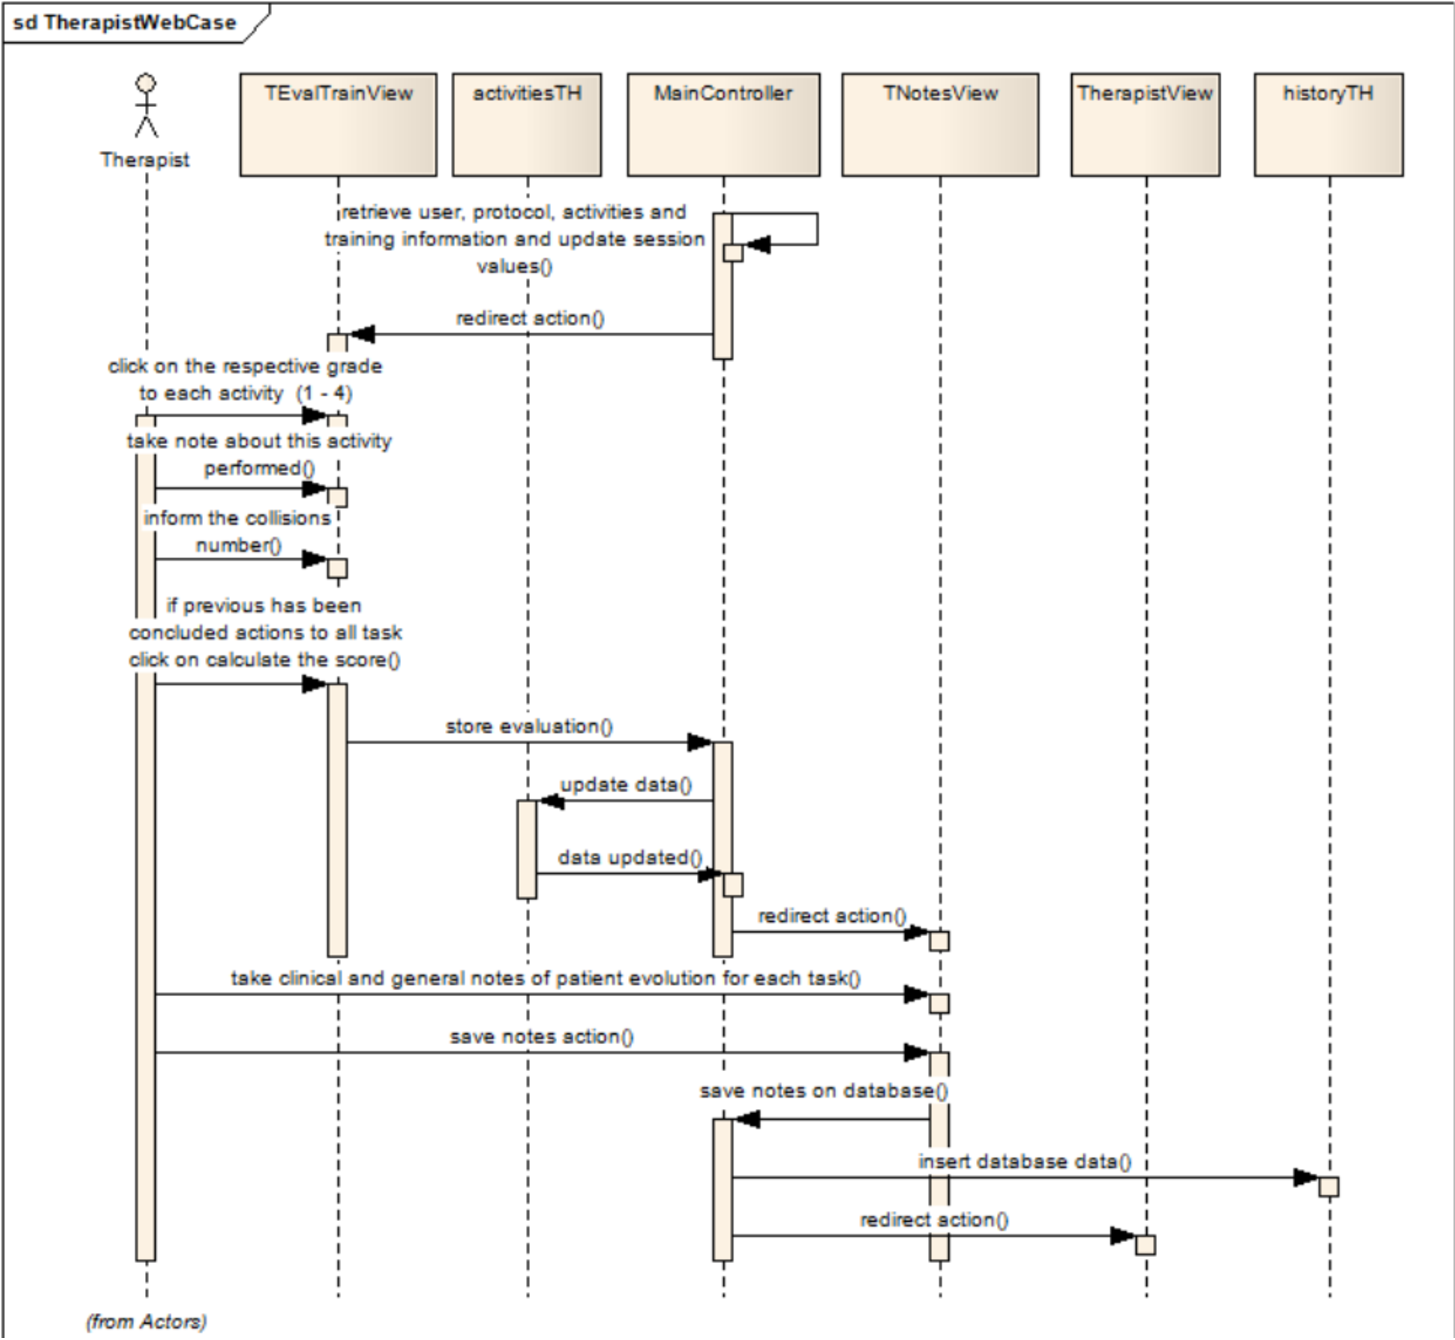
\includegraphics[width=0.7 \textwidth]{img/cap4/UMLSD-TherapistWebCase05}
\caption{Web training evaluate and notes view actions - Therapist UML-SD}
\label{fig:UMLSD-TherapistWebCase05}
\end{center}
\vspace{-20pt}
\end{figure} 

\subsubsection{User history accompaniment - Therapist  use case UML-SD}

The lastest therapist action SD is presented in Figure \ref{fig:UMLSD-TherapistWebCase06} that's to allow to preview the user evolution for each protocol performed.
 
\begin{figure}[!hbt]
\begin{center}
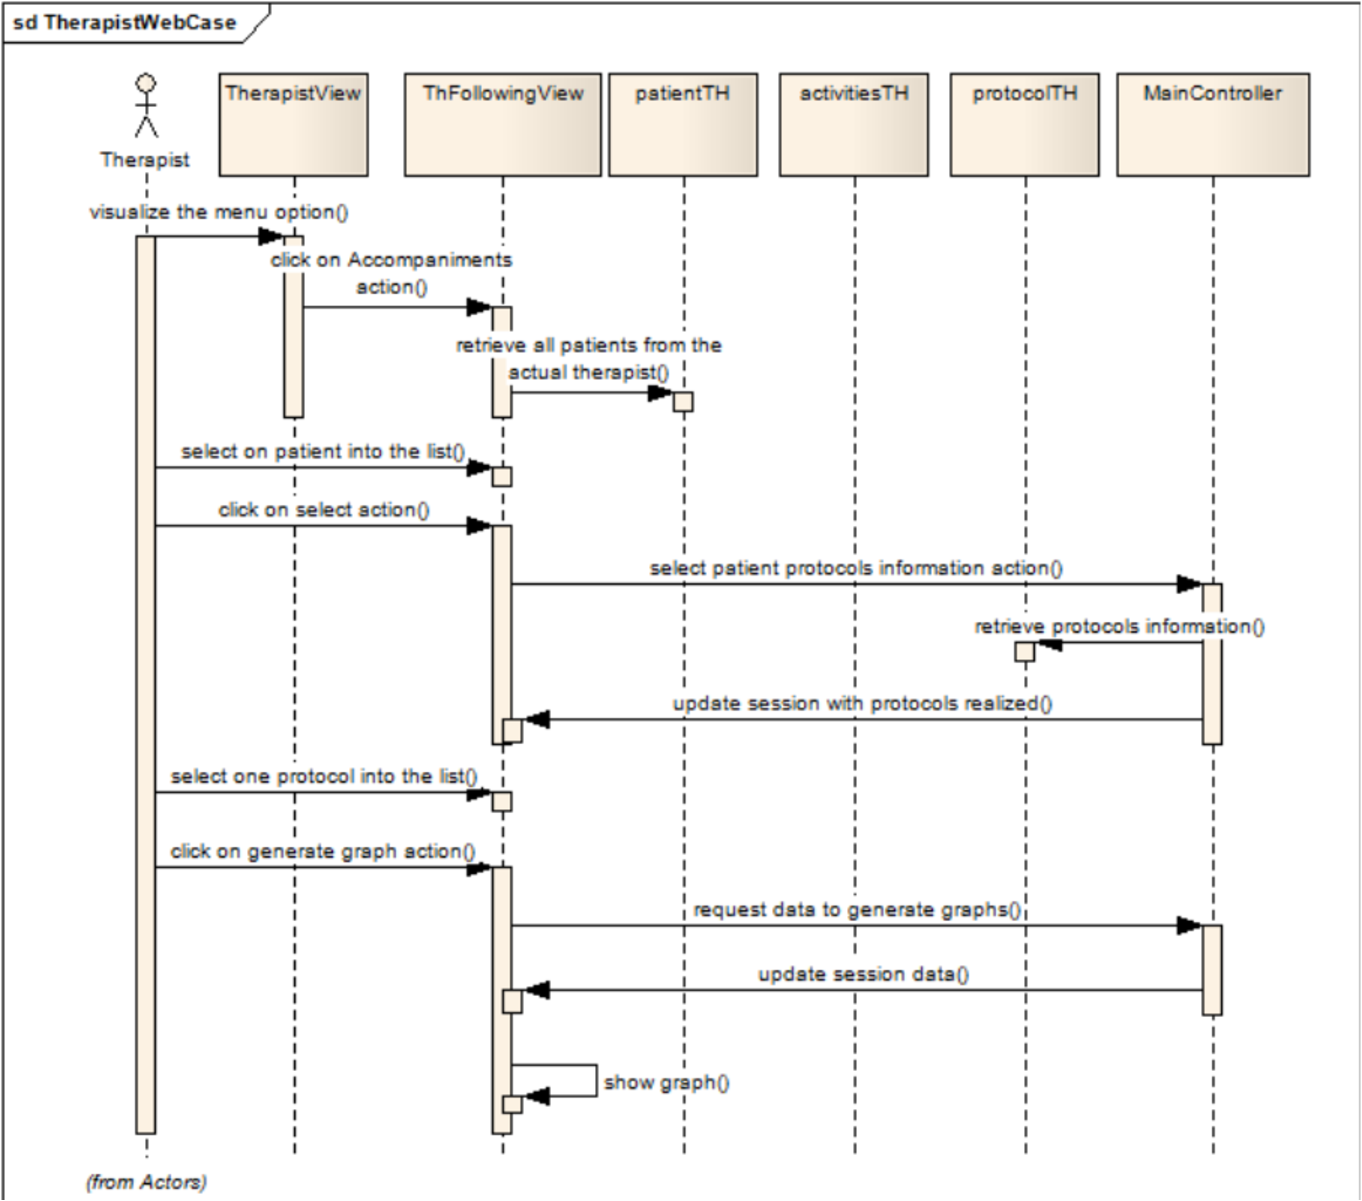
\includegraphics[width=0.7 \textwidth]{img/cap4/UMLSD-TherapistWebCase06}
\caption{Web user history accompaniment - Therapist UML-SD}
\label{fig:UMLSD-TherapistWebCase06}
\end{center}
\vspace{-20pt}
\end{figure} 

The therapist is allowed, at any time, using bar charts, highlighting the final protocol score and the auxiliary metrics defined. 


\section{Final considerations}

This chapter presents an AR-based Telerehabilitation environment for supporting the training of PW users, composed of three sites: patient, training, and therapist. In the training site, the resources and methods used to control the PW,  data channel and also video streaming using the WebRTC framework, was described. They are necessary to support remote interaction. From the patients' site, using an adapted USB joystick, the user will be able to control the PW remotely. The AR renderization on clients is processed based on markers to each frame received from the training site using WebRTC. The therapist can perform different tasks even apart of the training and patient site, simultaneously supported by the PMRT, that is a reliable assessment and protocol methodology and also tracks the user evolution using bar charts. Finally, the webserver application components were designed to support all these requirements, and in the end, based on therapist comments and survey filled out by the users, it is possible to have an evaluation of the proposed augmented Telerehabilitation architecture. In the next chapter, the respective implementation details will be presented.

